\begin{document}
\chapter{ABIG}
This Supplementary Material provides additional derivations, implementation details and results. More specifically: 
\begin{itemize}[noitemsep]

    \item Section \ref{ap:method} proposes derivations, implementation details and analysis related to our method.
    \begin{itemize}[noitemsep]
        \item Subsection \ref{ap:sec_sketch} provides additional diagrams illustrating the ABP problem and its position with respect to related settings.
        \item Subsection \ref{ap:method_analytic} proposes the full derivation of the agents' MDP.
        \item Subsection \ref{ap:algo} proposes our methods pseudo-code, algorithmic implementation details (for BC and MCTS), hyper-parameters and compute resources.
        \item Subsection \ref{sup:sec_res_toy} proposes analysis that explore our method's learning mechanisms.
        \item Subsection \ref{ap:sec_related_work} discusses the differences between \abp and Hierarchical/Feudal Reinforcement Learning.
    \end{itemize}
    \item Section \ref{ap:sup_res} provides additional results.
    \begin{itemize}[noitemsep]
        \item Subsection \ref{ap:results_bw} monitors the builder's behavior properties as training progresses.
        \item Subsection \ref{ap:baselines} compares our method to additional baselines.
        \item Subsection \ref{sup:sec_res_dict_size} analyses the impact of the vocabulary size on the learning performance. 
    \end{itemize}
\end{itemize}

% % Add the appendix text to the document TOC
% \part{\textsc{Supplementary Material}} % Start the appendix part
% \addcontentsline{toc}{paragraph}{Appendix}
% \parttoc % Insert the appendix TOC

\section{Supplementary Methods}
\label{ap:method}

\subsection{Supplementary Sketches}
\label{ap:sec_sketch}
\begin{figure}[h!]
    \centering
    \begin{tabular}{cc}
    \multicolumn{2}{c}{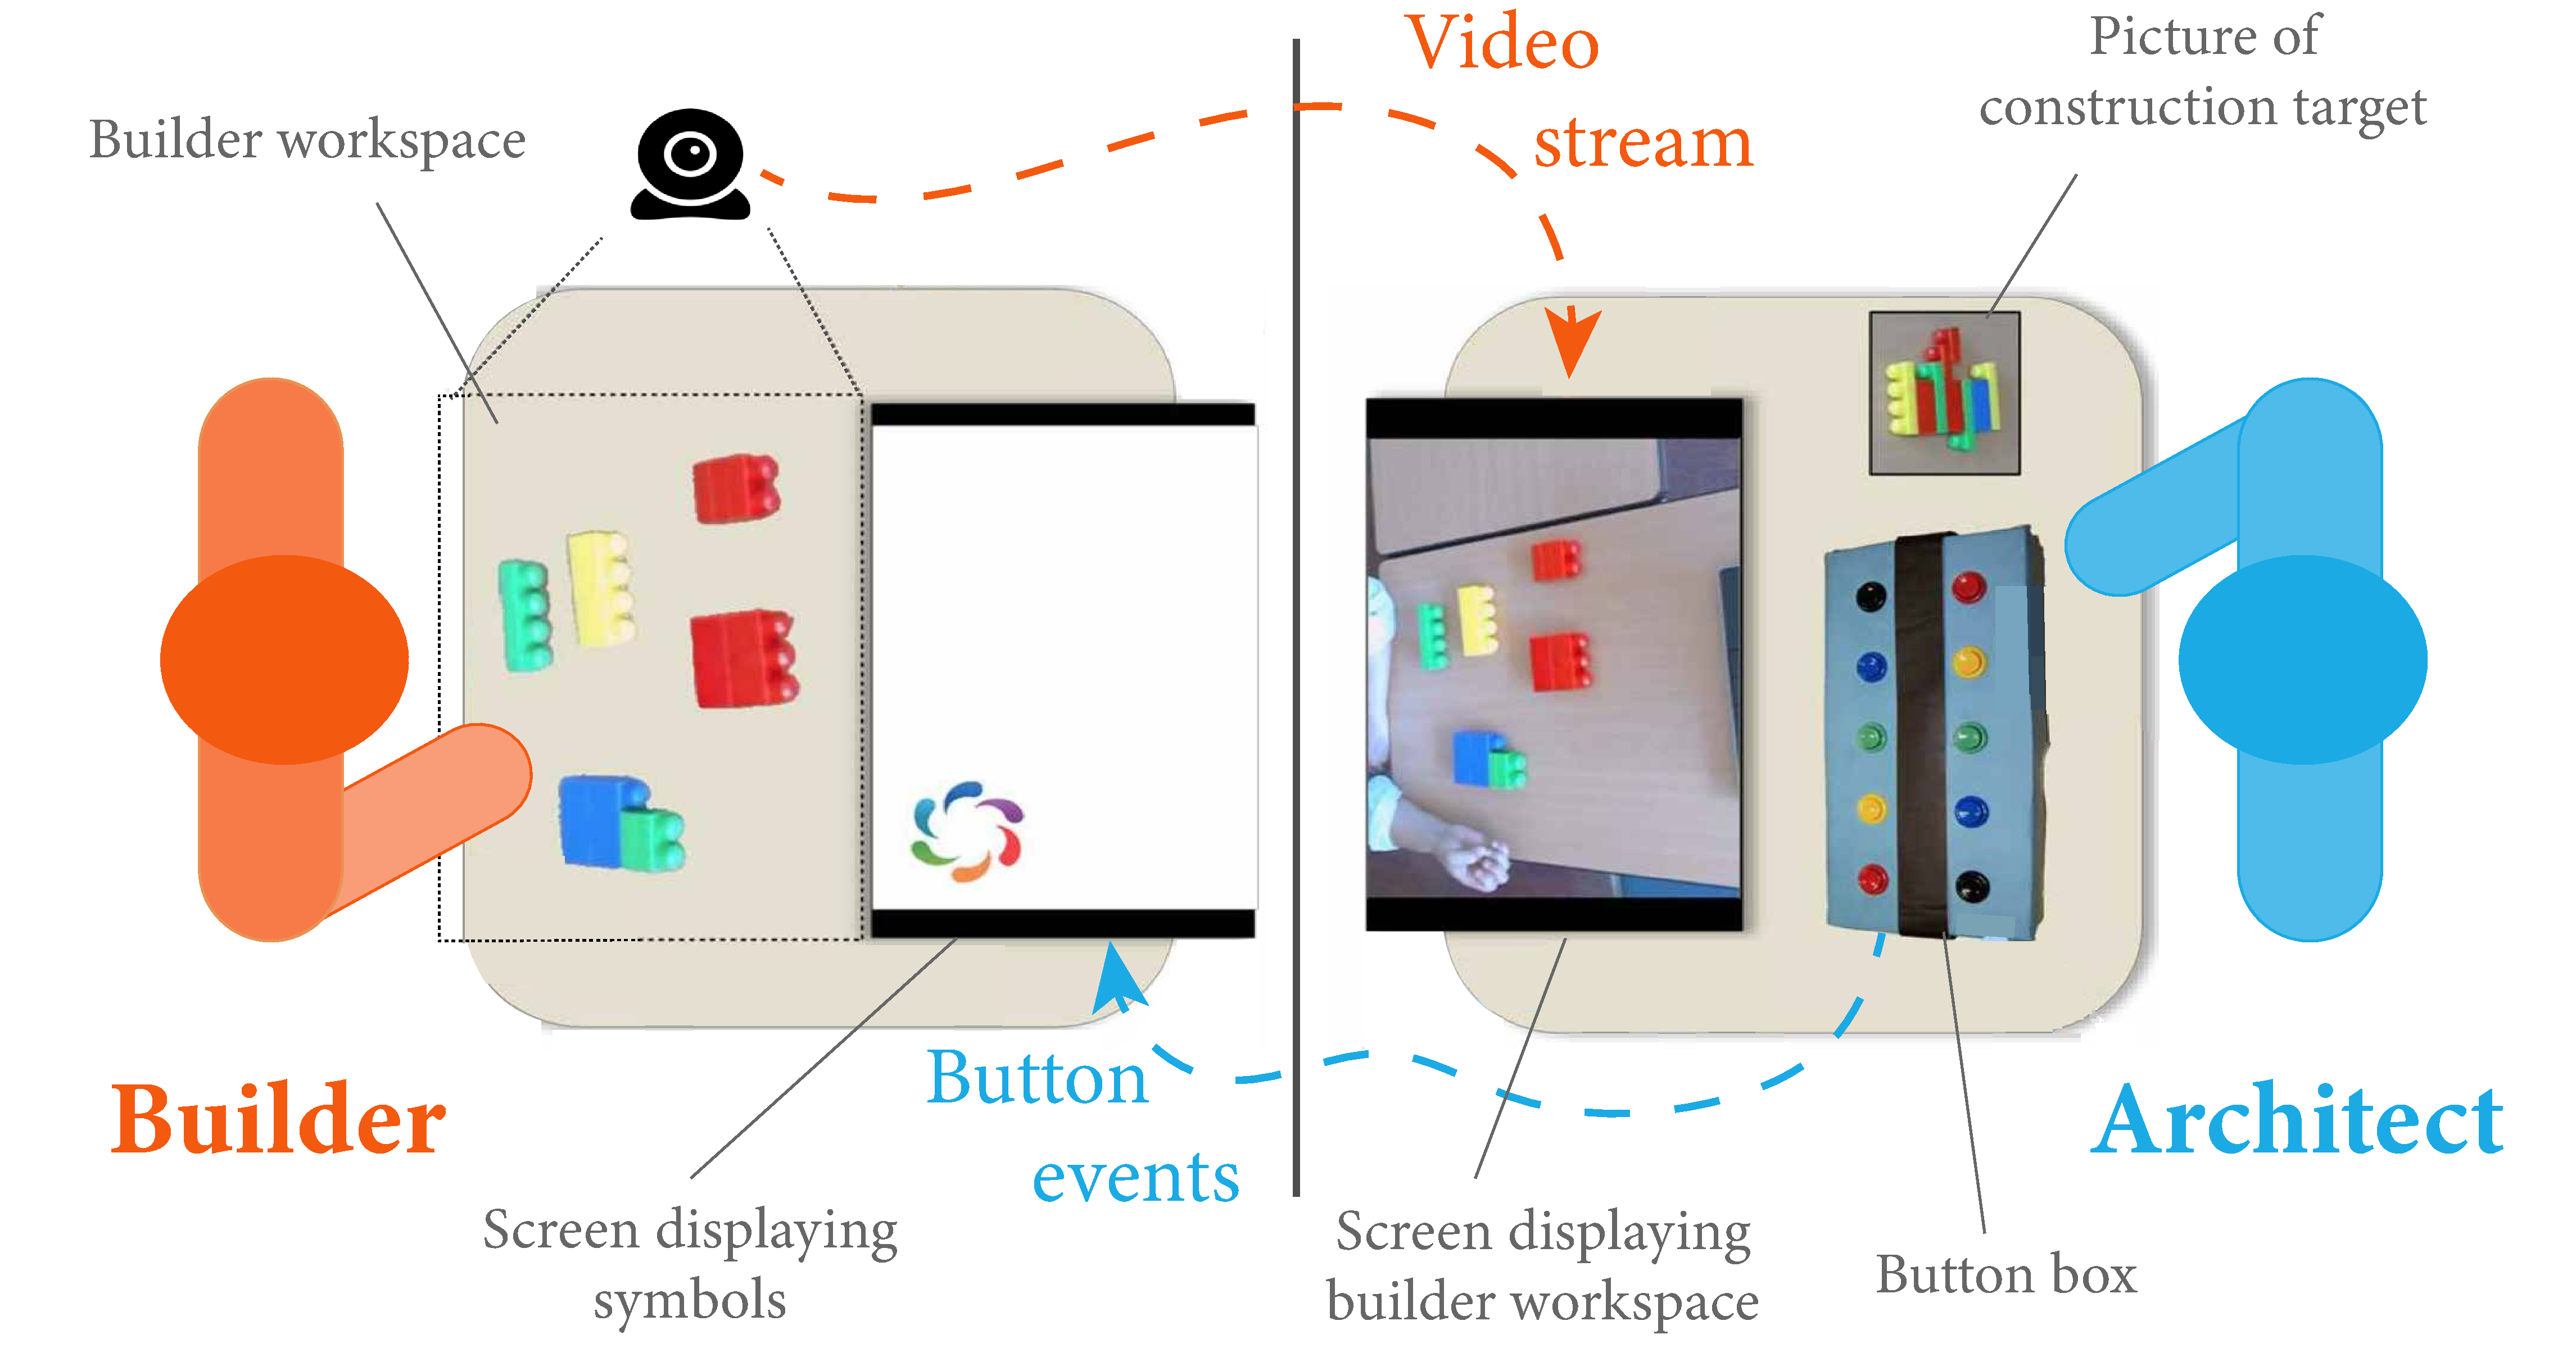
\includegraphics[width=0.5\textwidth]{abig/cocogame_horizontal.pdf}}\\
    \multicolumn{2}{c}{\small (a)}\\
 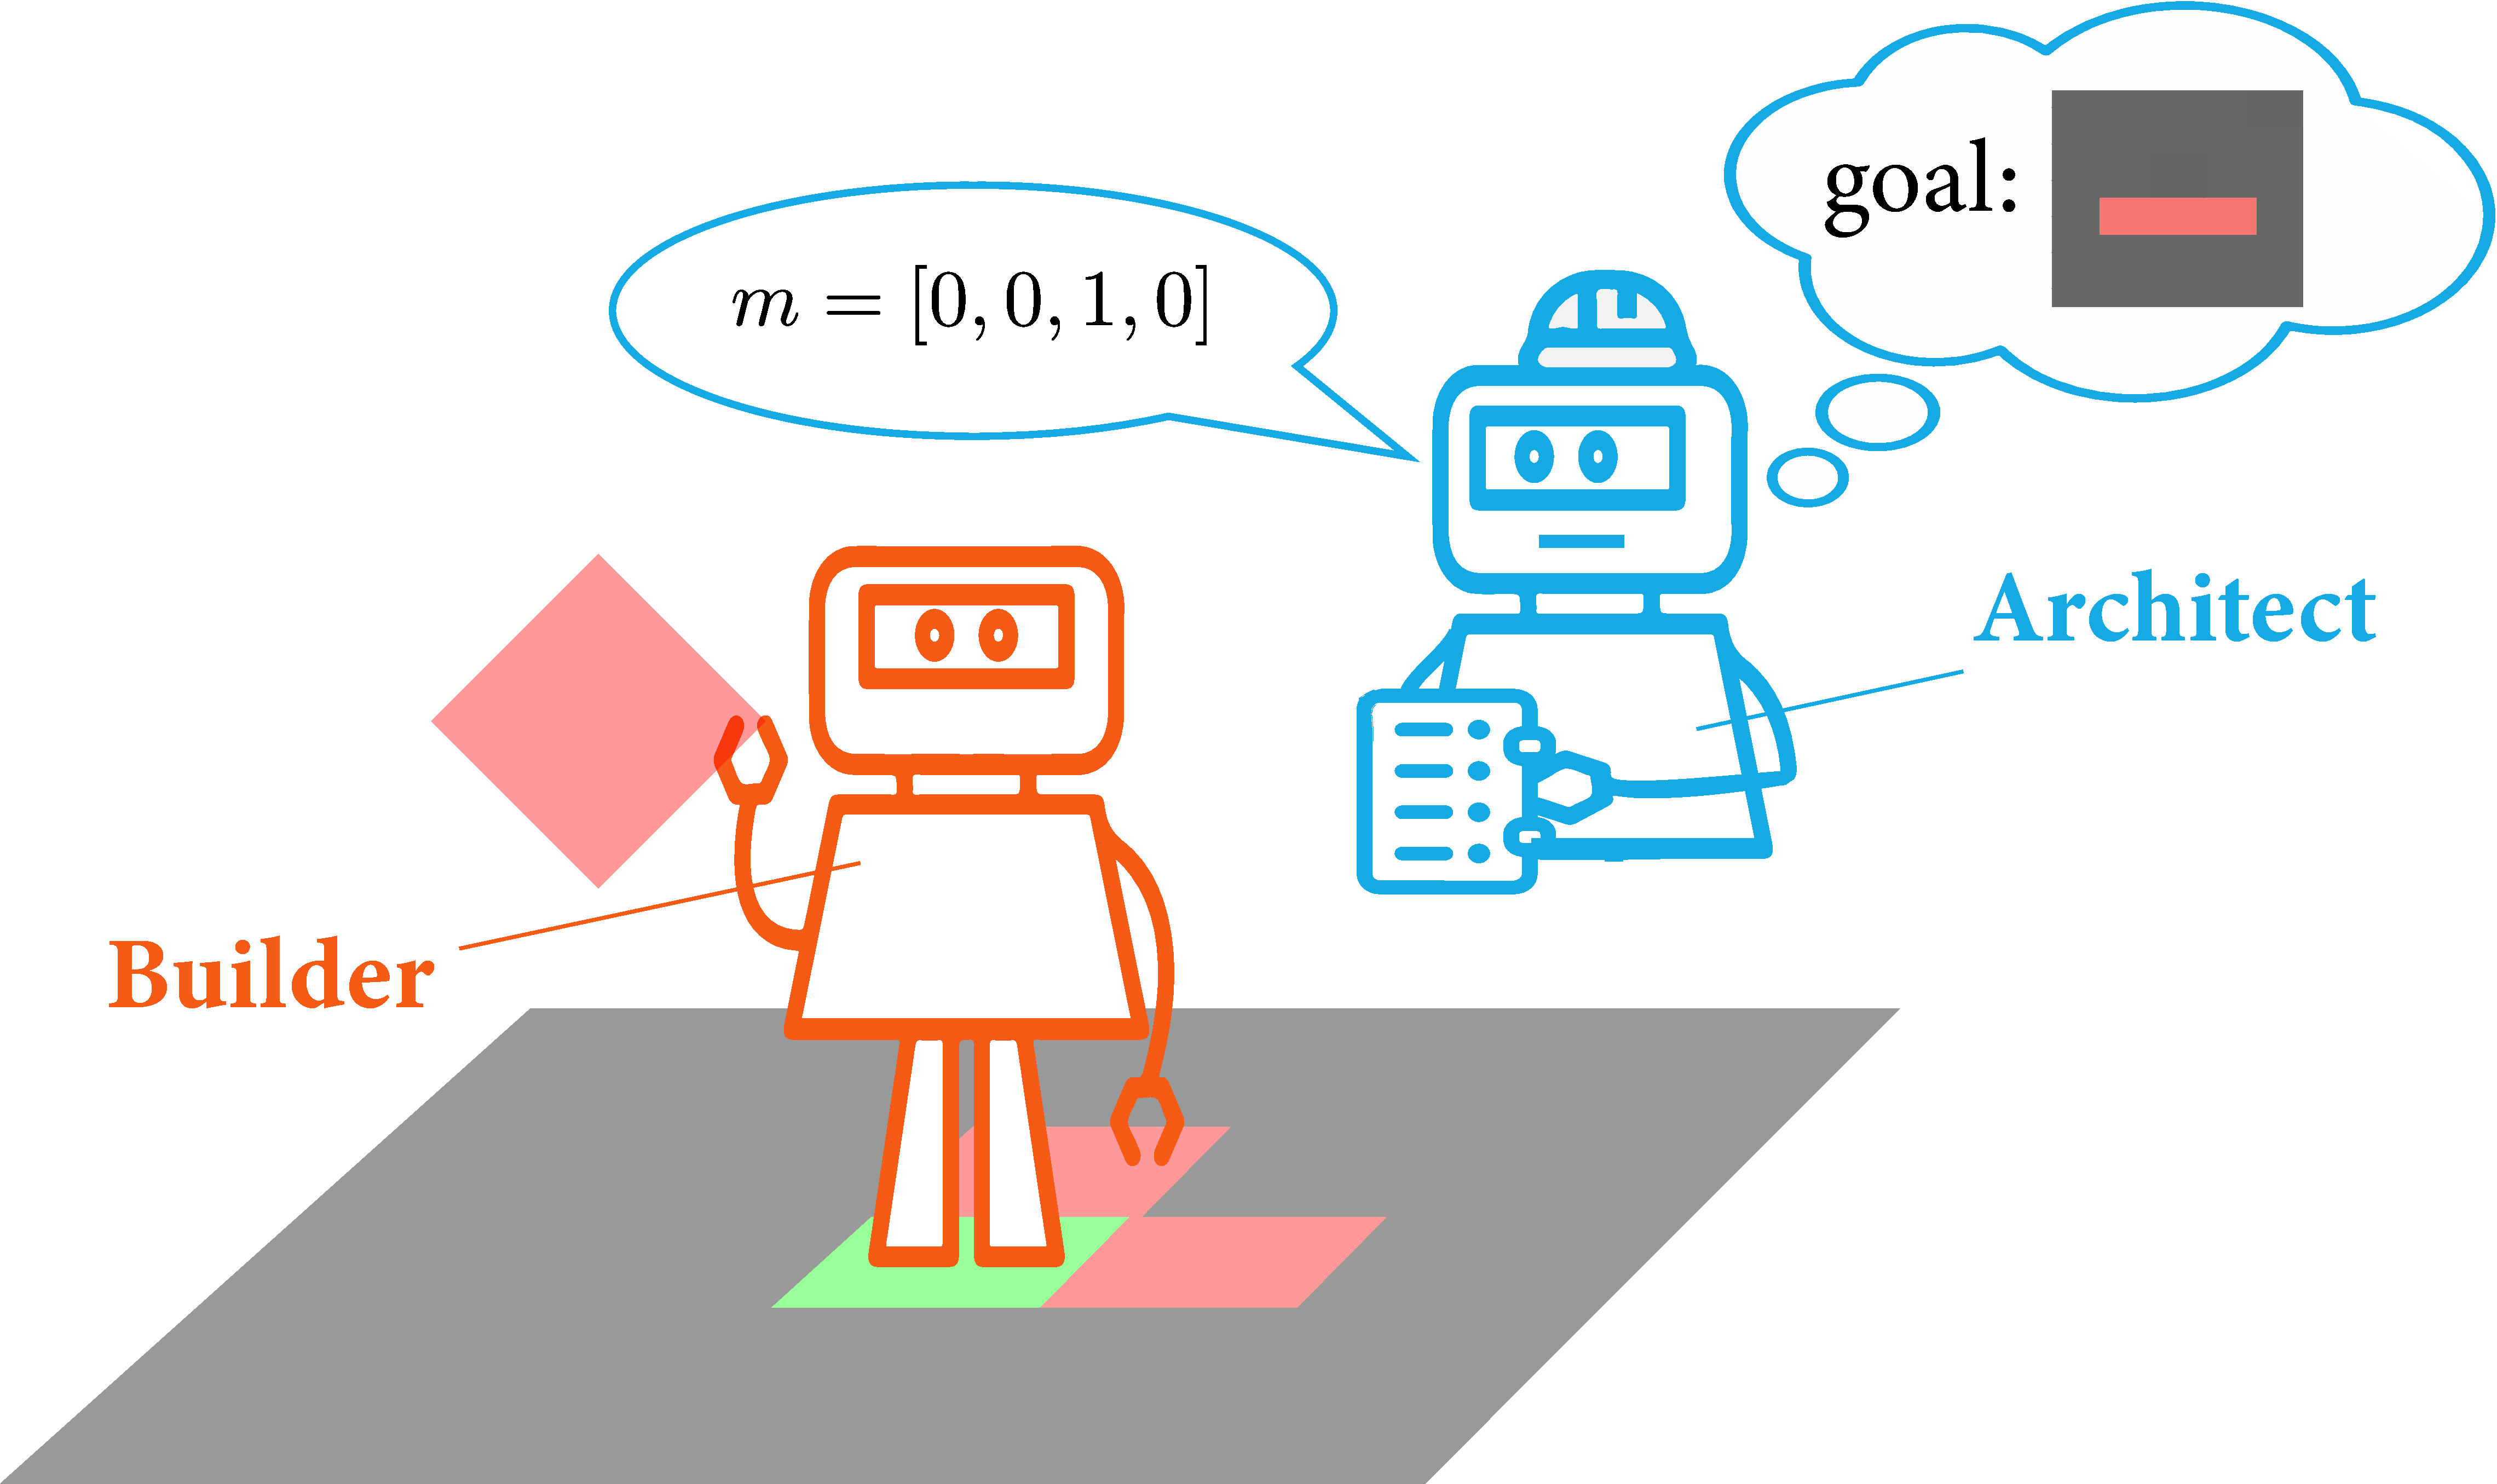
\includegraphics[width=0.45\textwidth]{abig/high_level_figure}    &  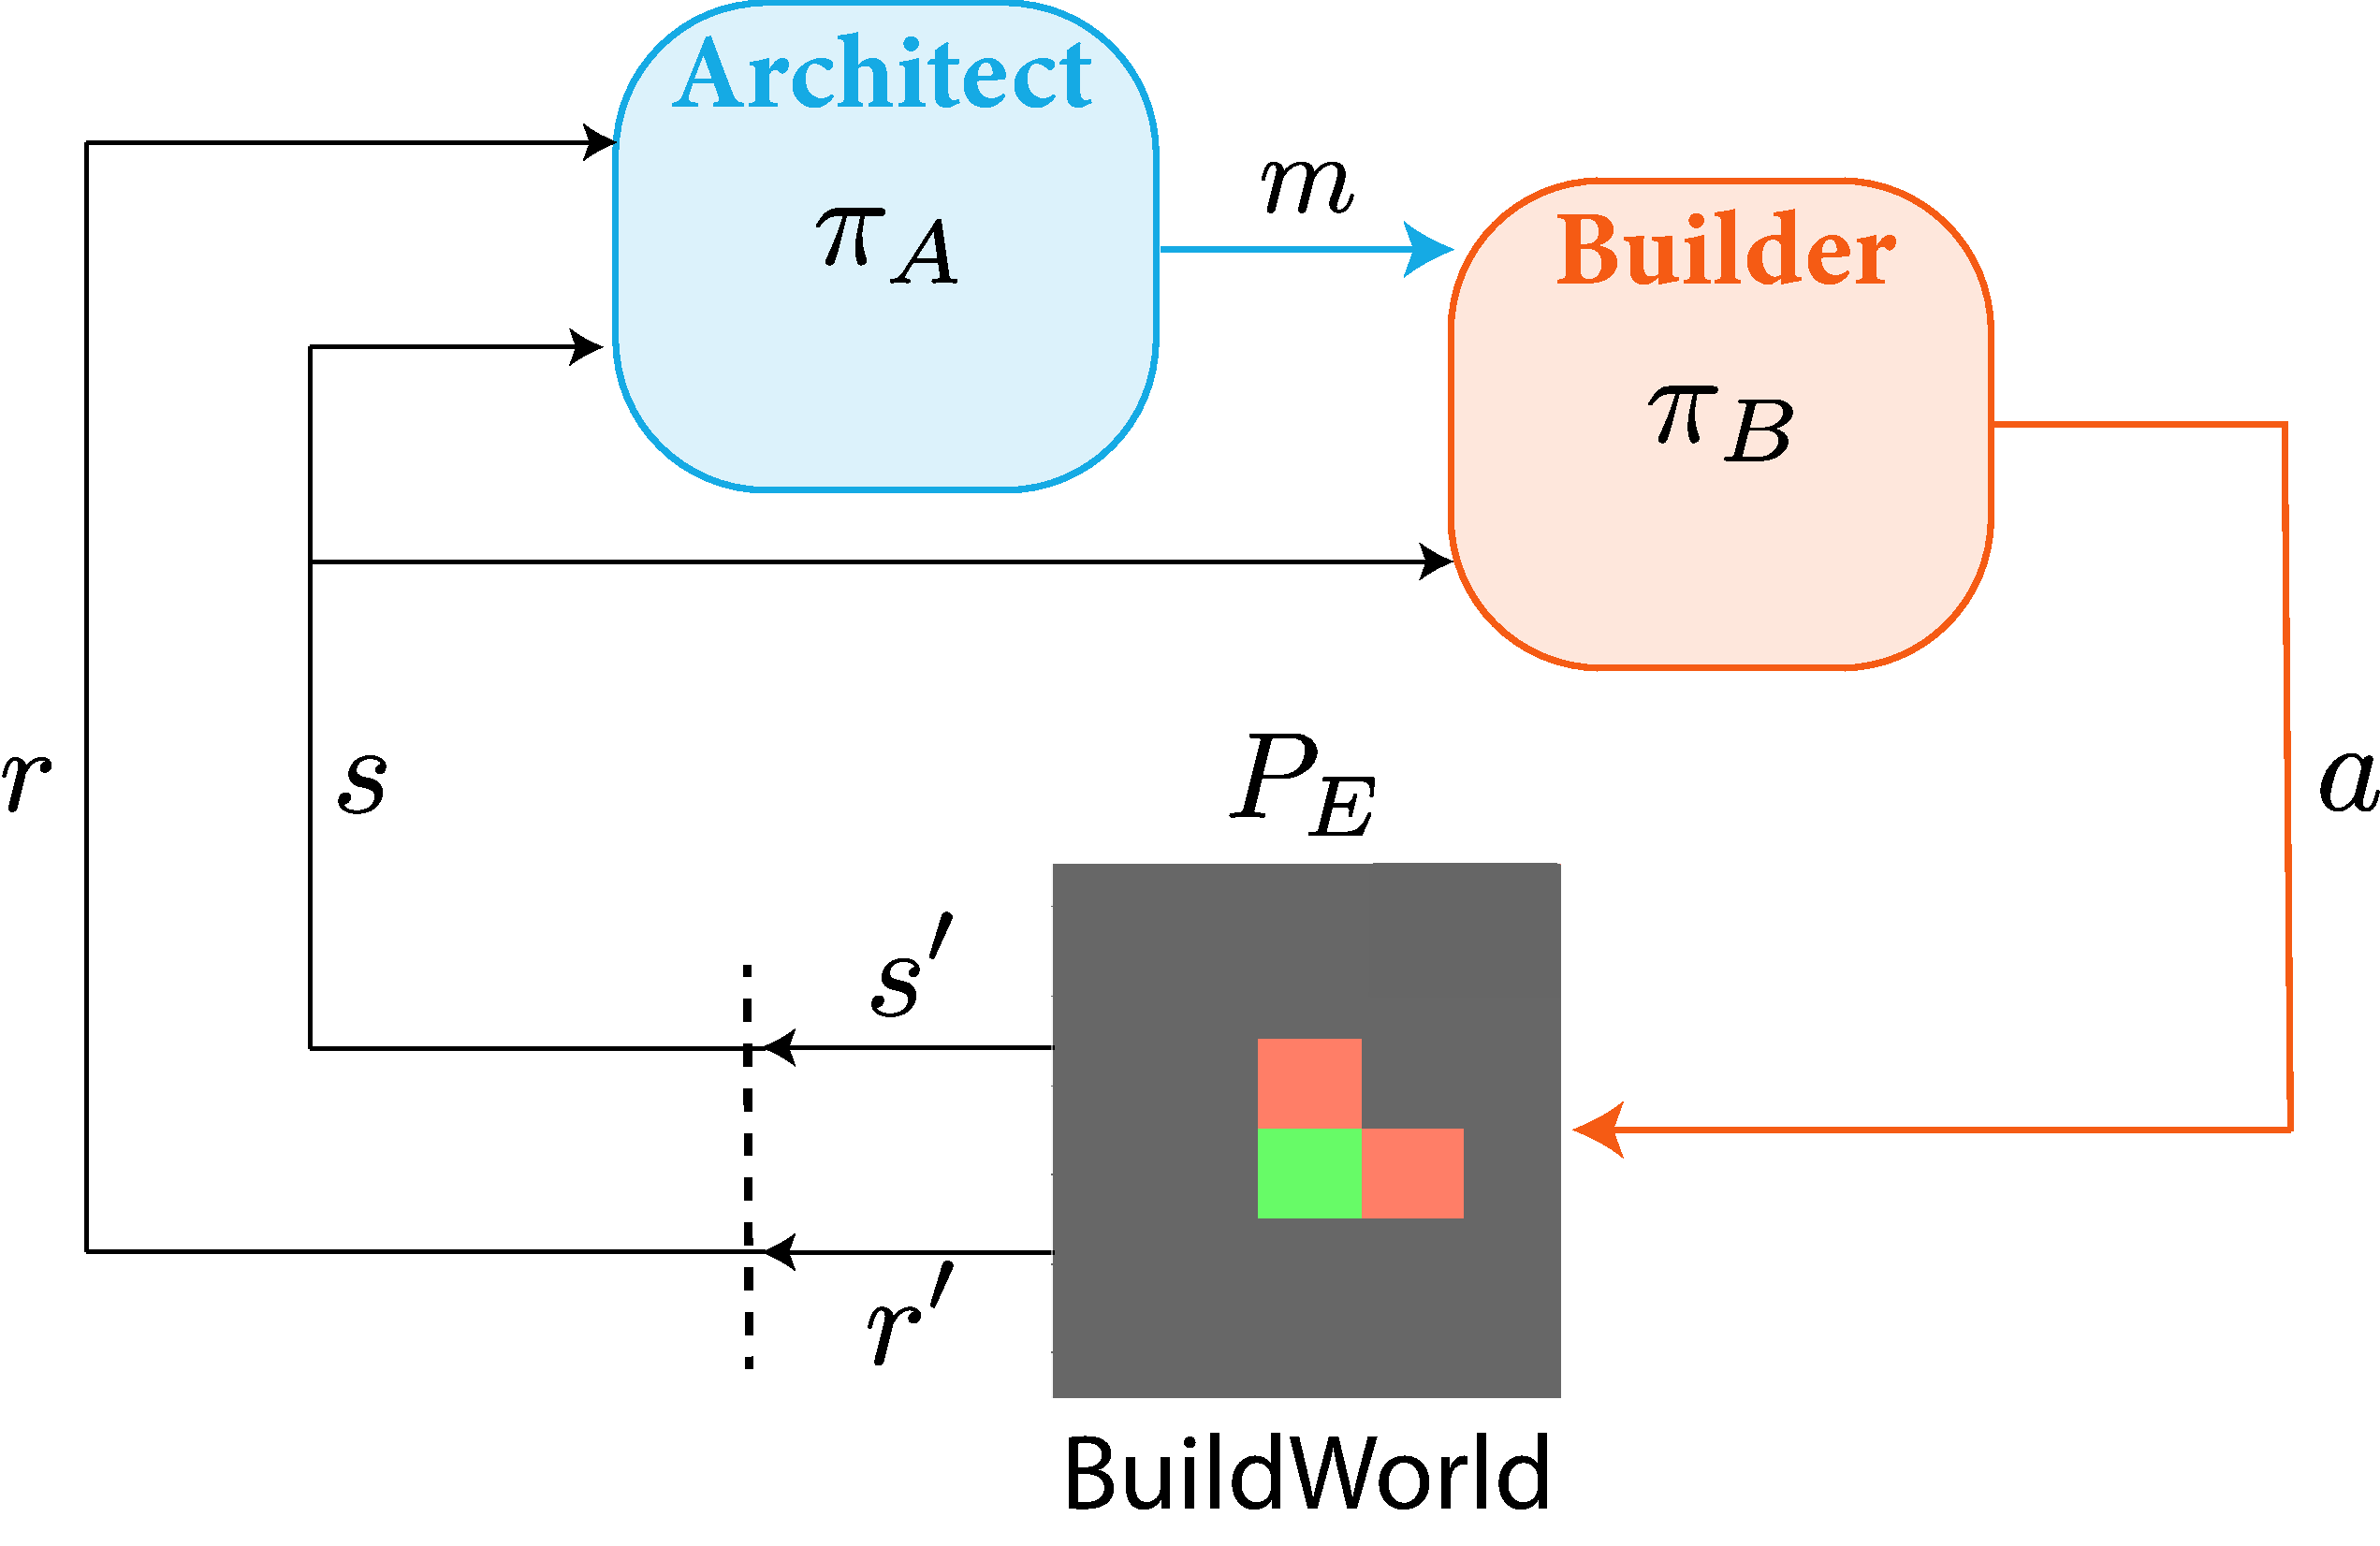
\includegraphics[width=0.4\textwidth]{abig/agent_diagram_v2} \\
    \small (b) & \small(c)
    \end{tabular}
    \caption{\small (a) \textbf{Schematic view of the CoCo Game.} The architect and the builder should collaborate in order to build the construction target while located in different rooms. The architecture has a picture of the target while the builder has access to the blocks. The architect monitors the builder workspace via a camera (video stream) and can communicate with the builder only through the use of 10 symbols (button events). (b) \textbf{Schematic view of the Architect-Builder Problem. } The architect must learn how to use messages to guide the builder while the builder needs to learn to make sense of the messages in order to be guided by the architect. (c) \textbf{Interaction diagram between the agents and the environment in our proposed \abp.} The architect communicates messages ($m$) to the builder.  Only the builder can act ($a$) in the environment. The builder conditions its action on the message sent by the builder ($\pib(a|s,m)$). The builder never perceives any reward from the environment}
    \label{fig:sup_diagram}
\end{figure}

\begin{figure}[h!]
    \centering
    \begin{tabular}{cccc}
    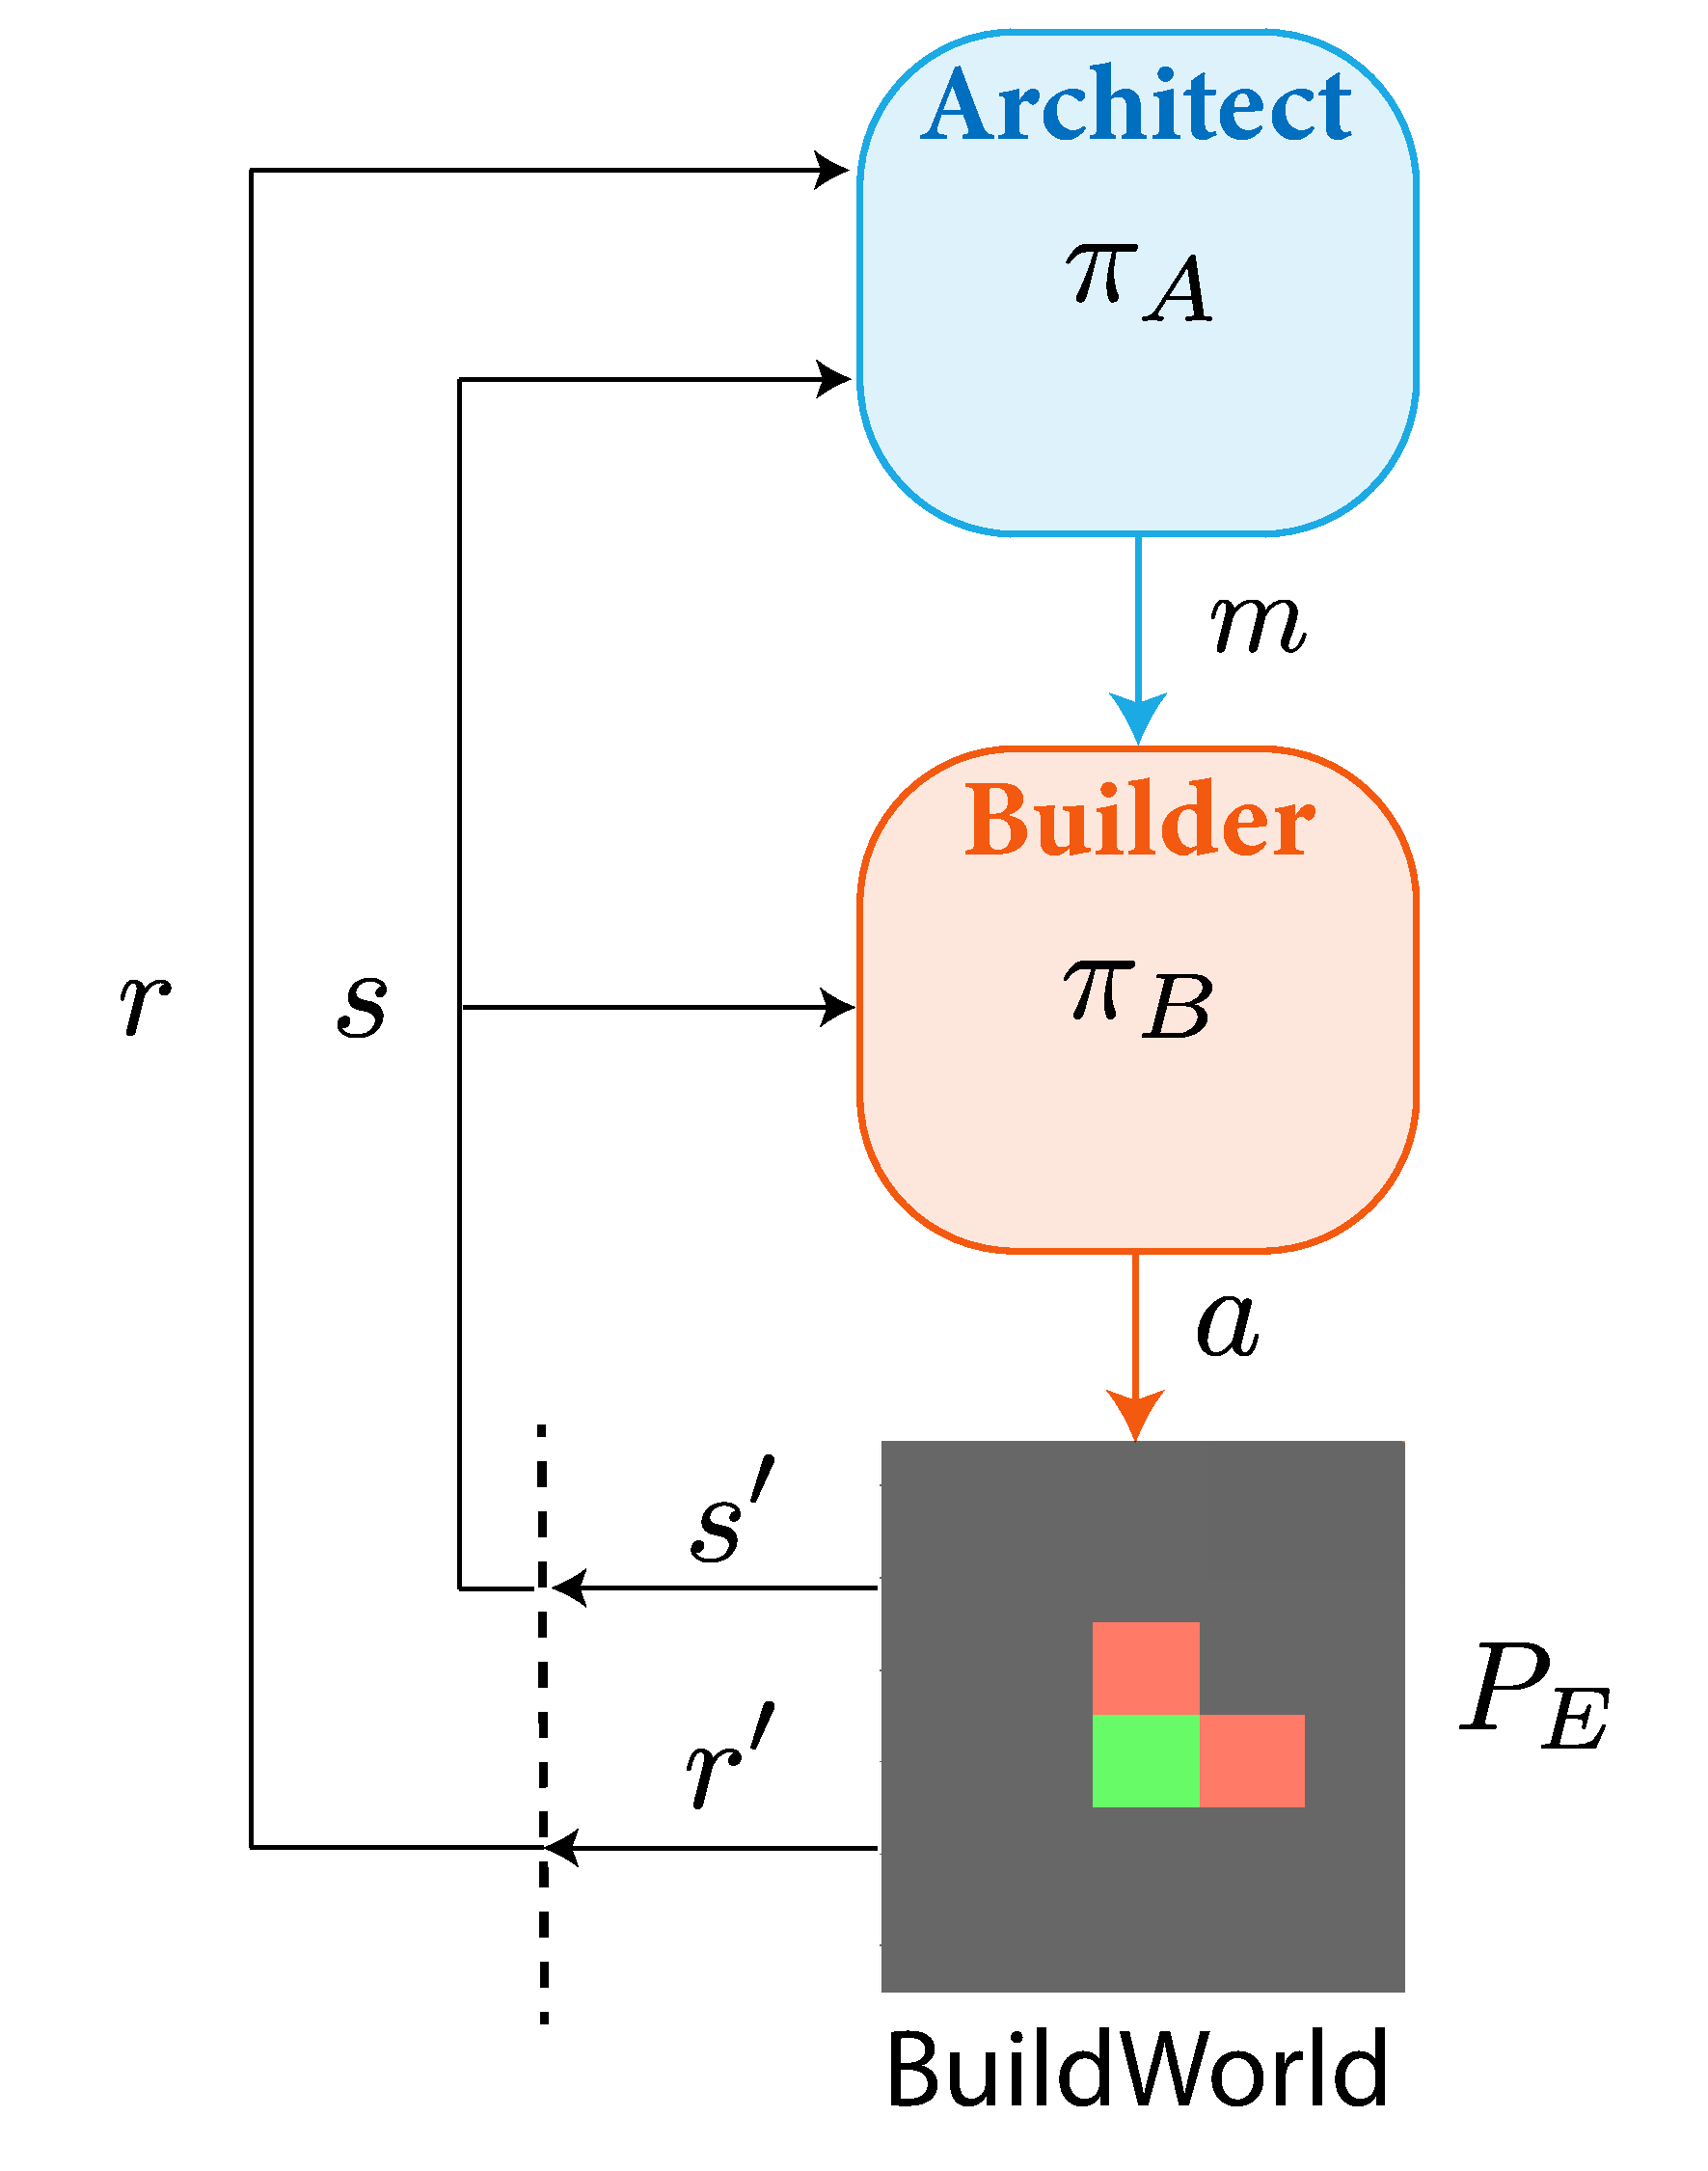
\includegraphics[width=0.22\textwidth]{abig/abp_v.pdf} & 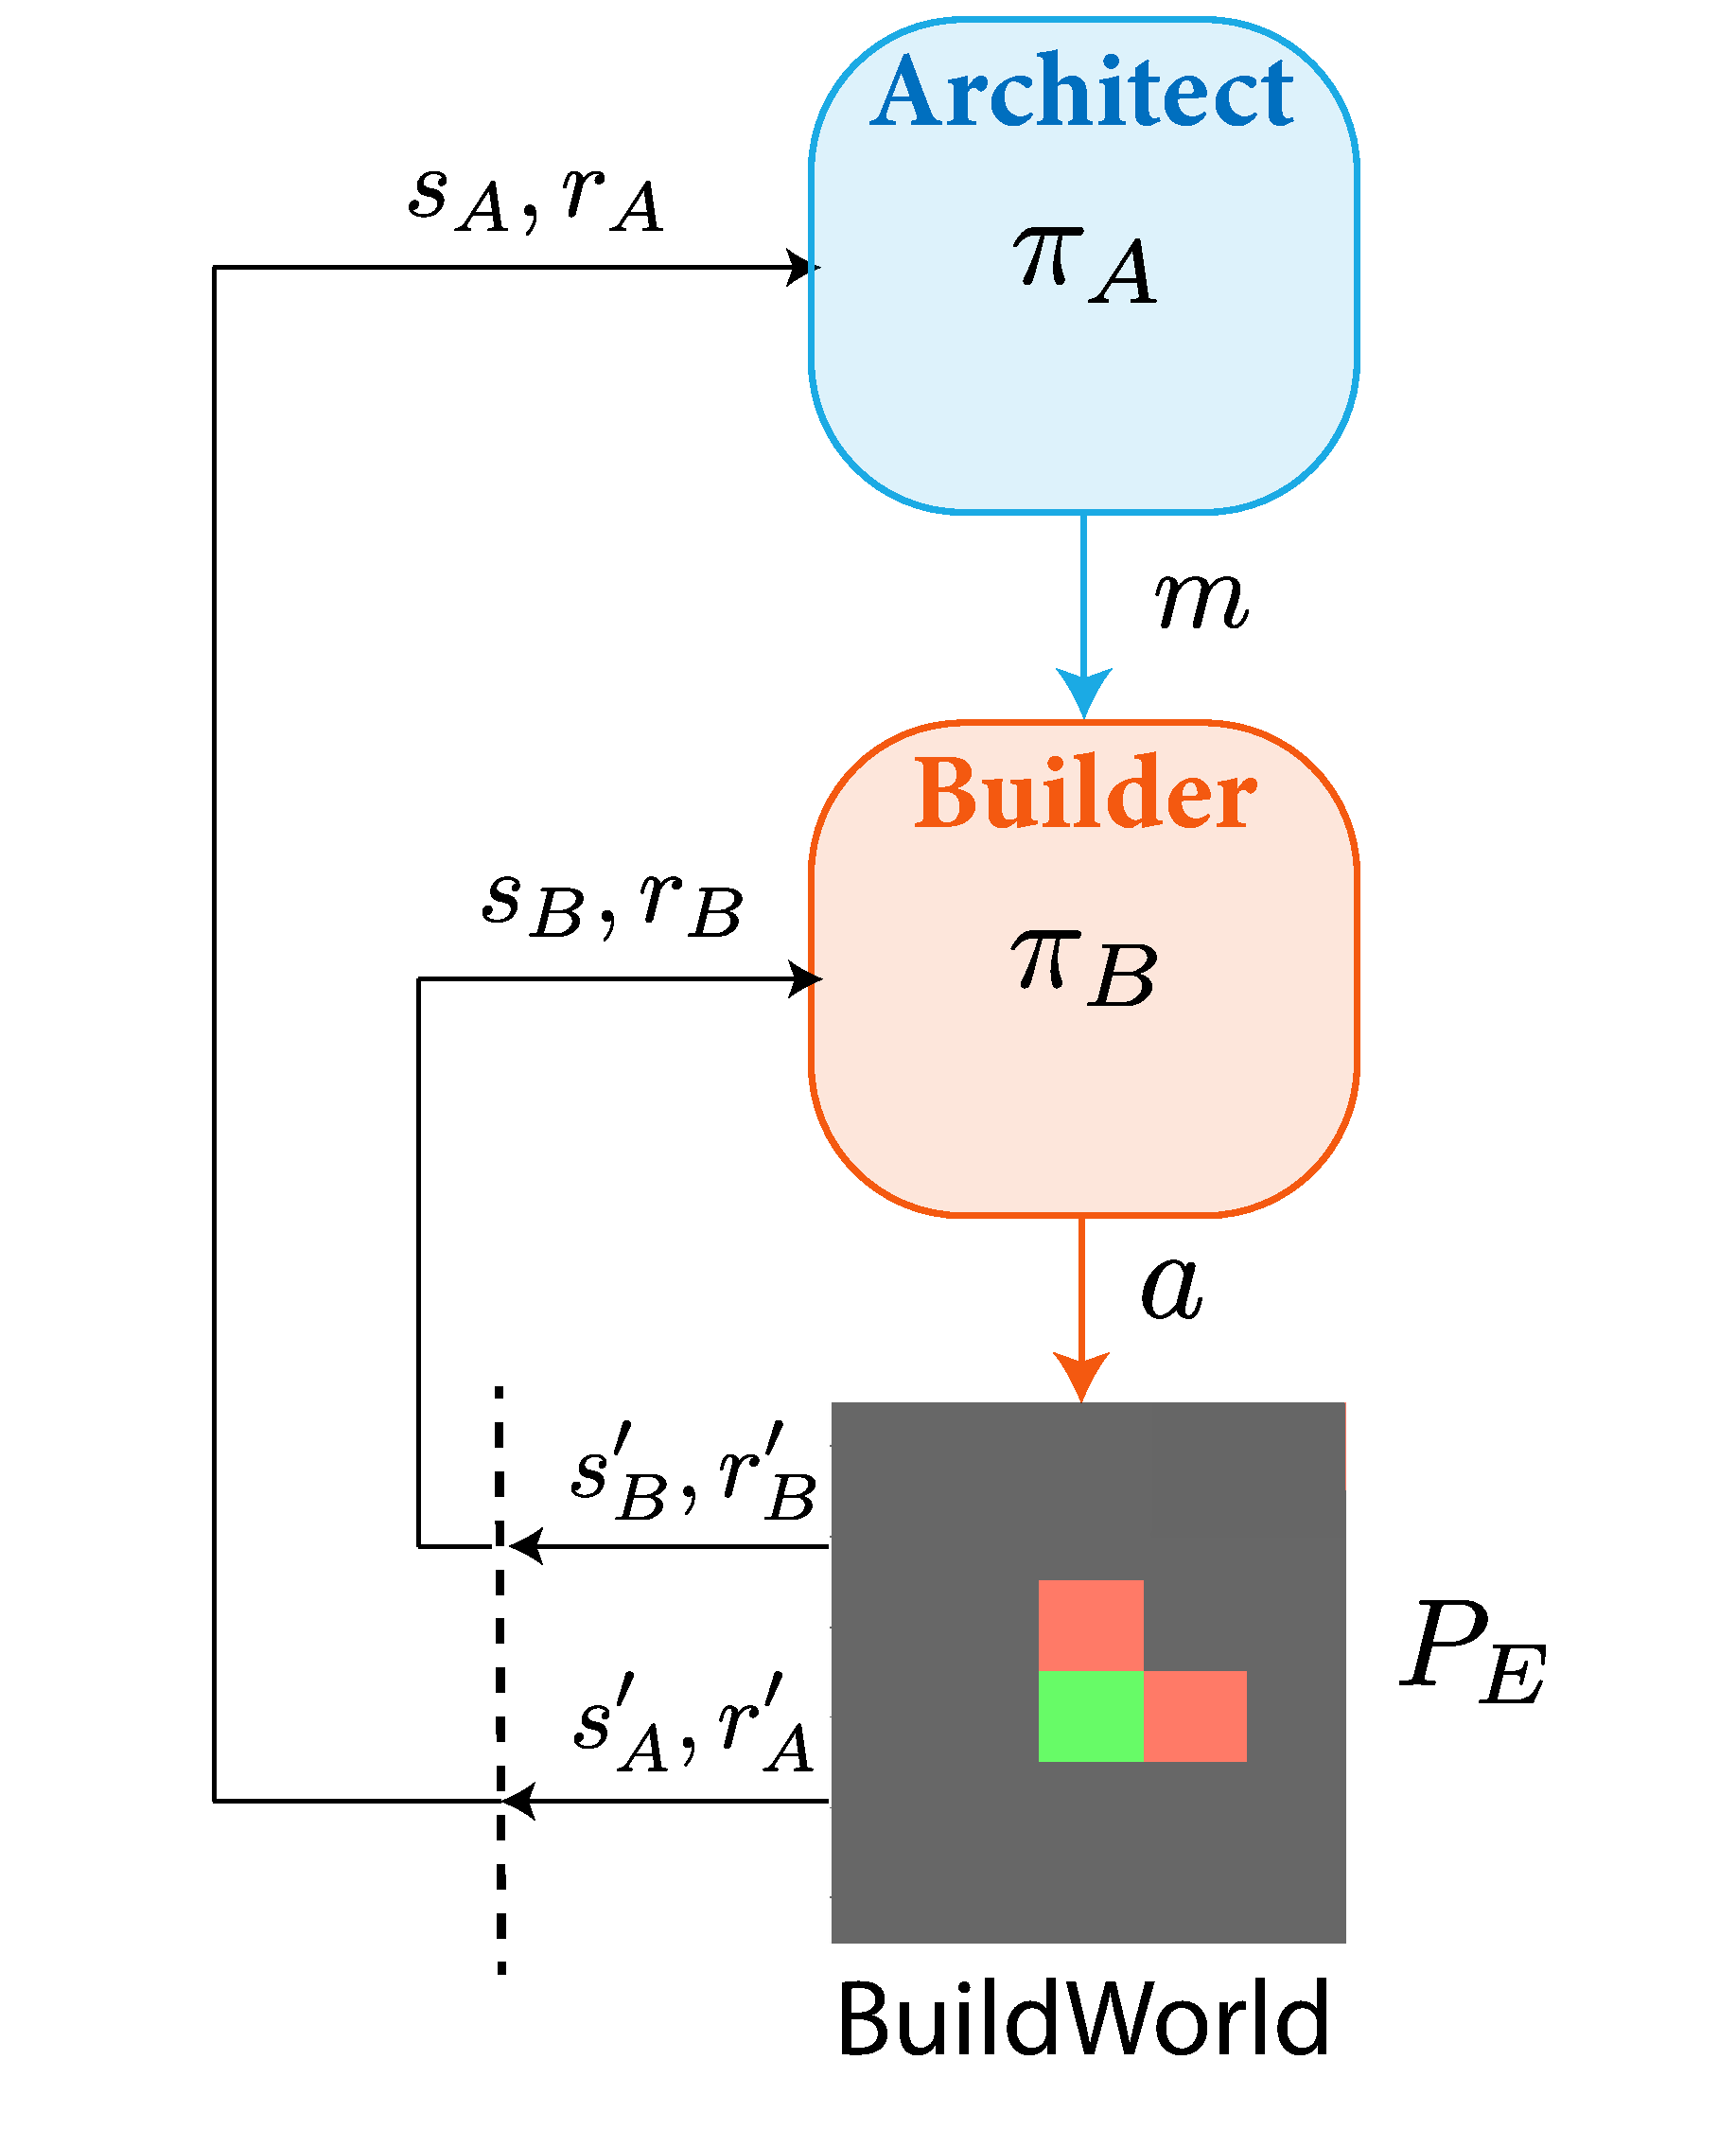
\includegraphics[width=0.23\textwidth]{abig/abp_marl.pdf} &  \multicolumn{2}{c}{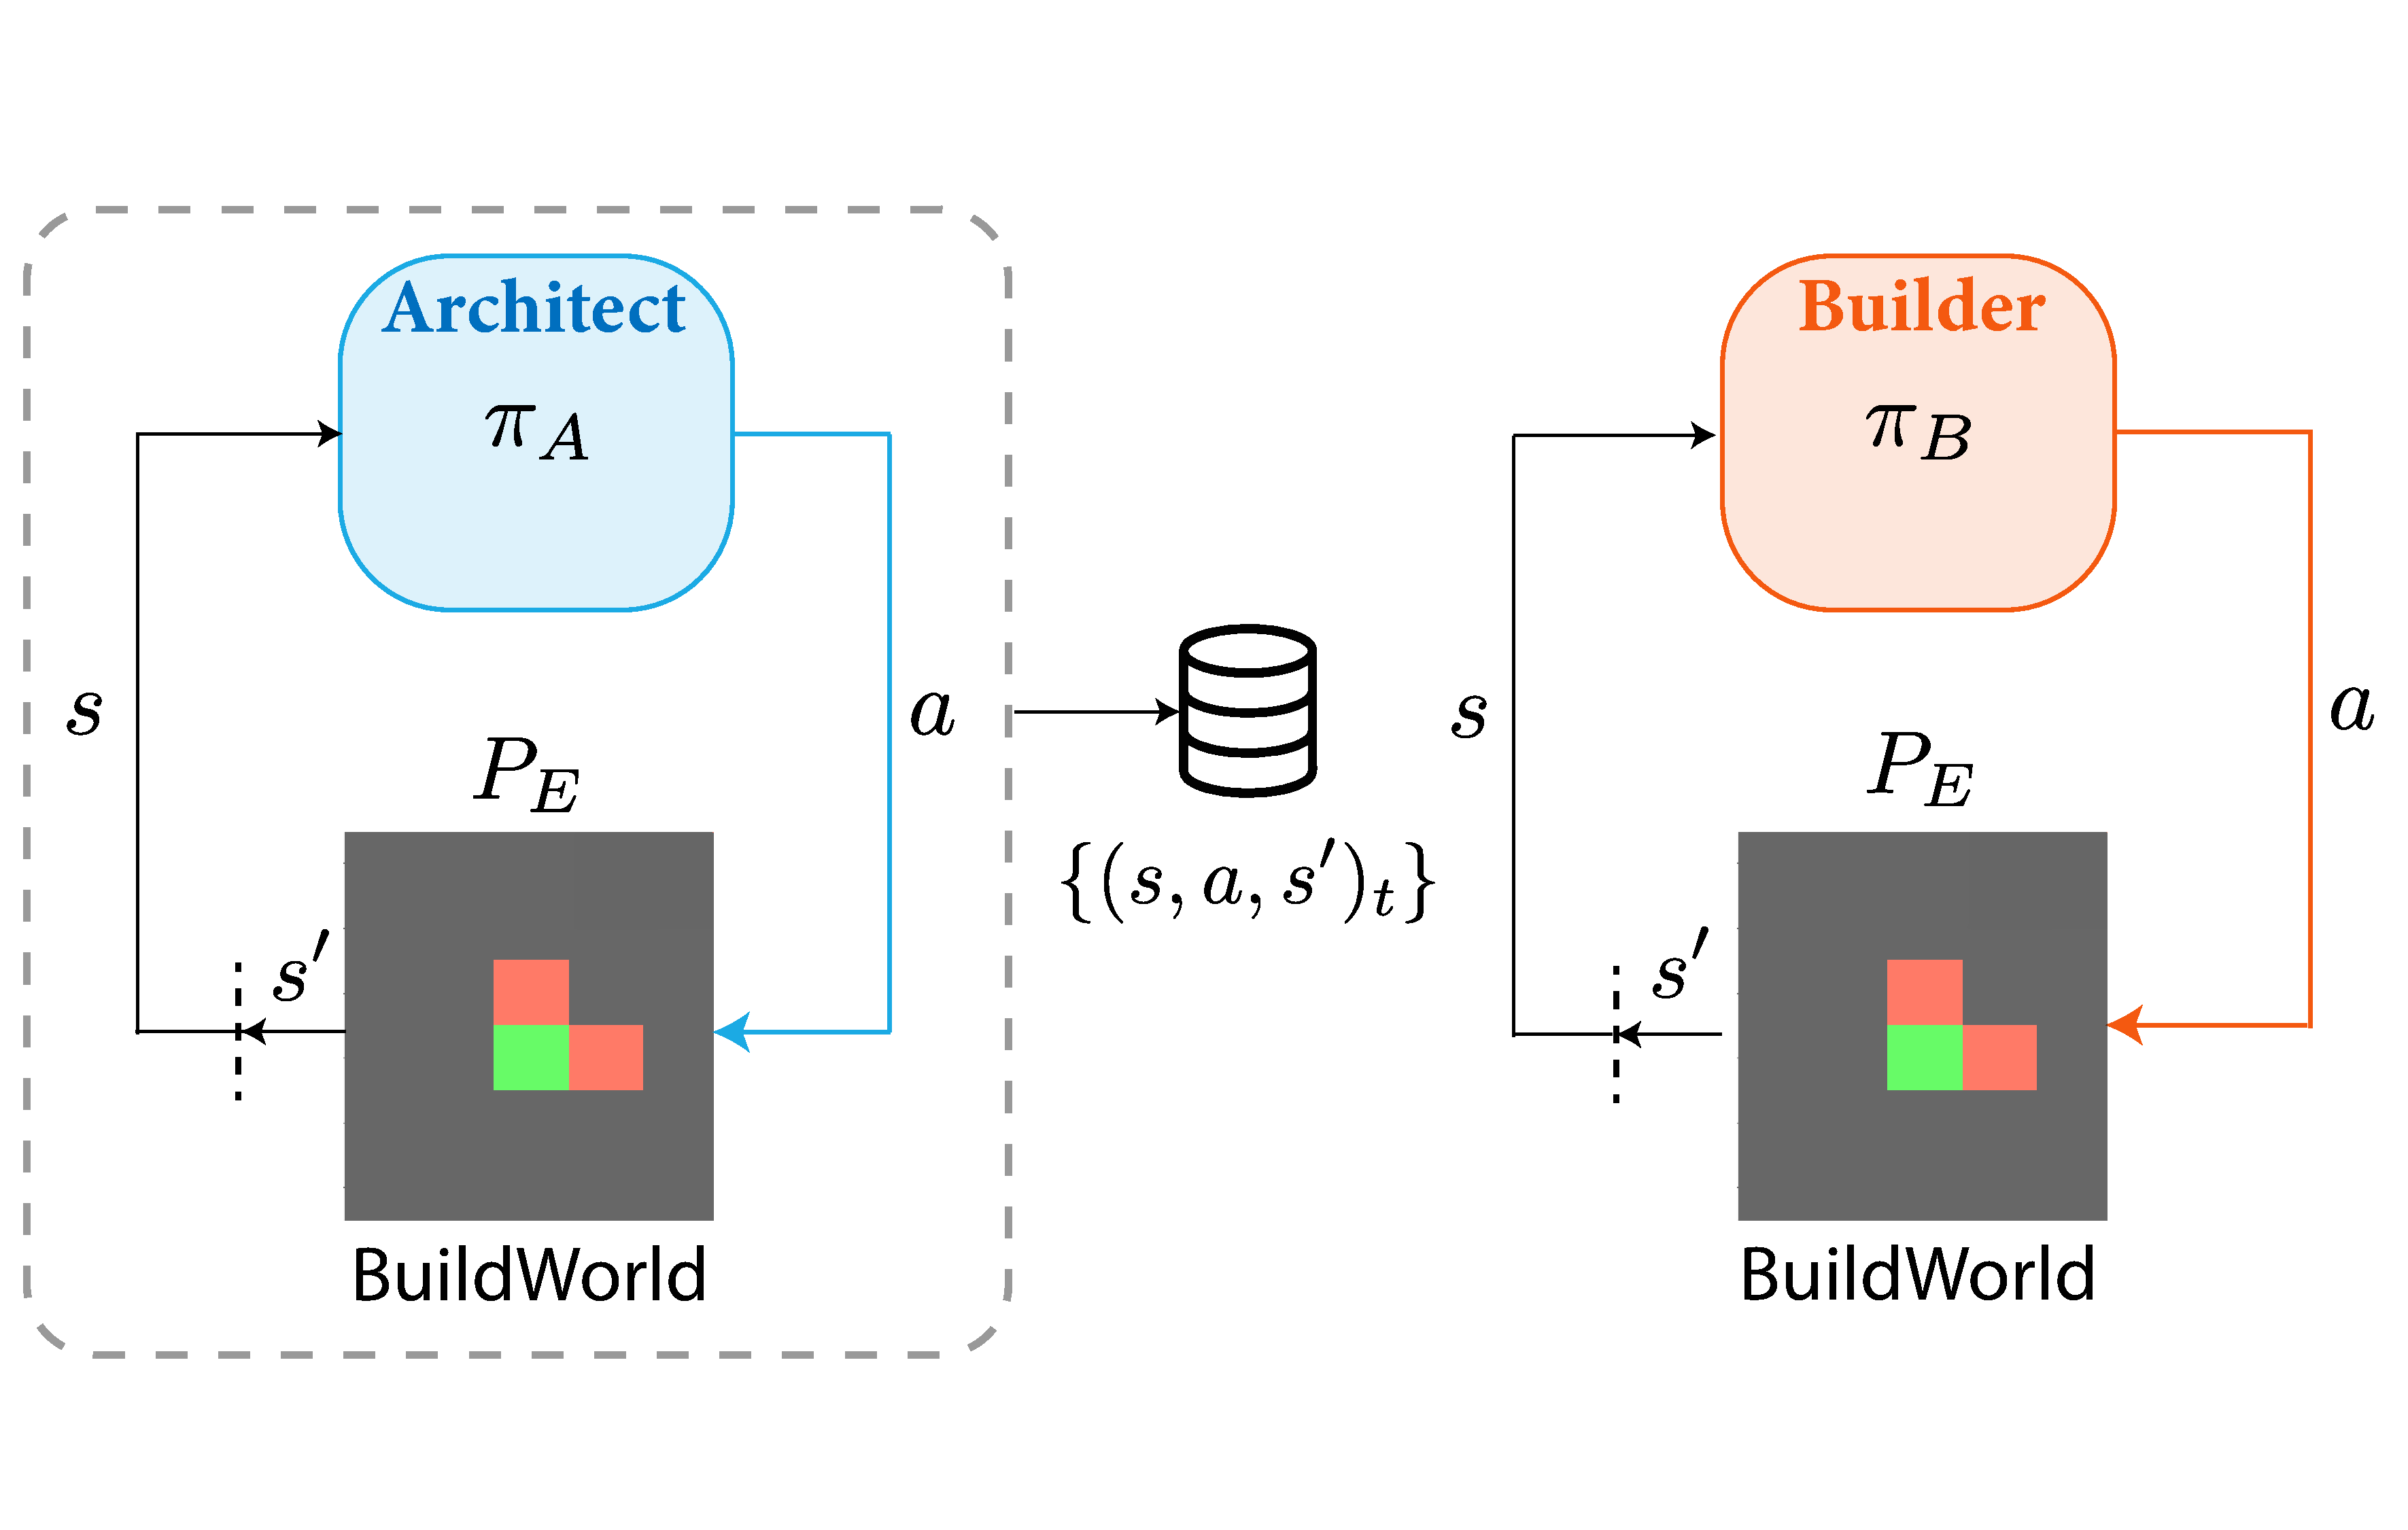
\includegraphics[width=0.46\textwidth]{abig/abp_irl.pdf}}\\
    \small (a) & \small(b) & \multicolumn{2}{c}{\small(c)}
    \end{tabular}
    \caption{\small (a) \textbf{Vertical view of the interaction diagram between the agents and the environment in our proposed ABP. } Only the architect perceives a reward signal $r$; (b) \textbf{Interaction diagram for a standard MARL modelization. } Both the architect and the builder have access to environmental rewards $r_A$ and $r_B$. Which would contradict the fact that the builder ignores everything about the task at hand; (c) \textbf{Inverse Reinforcement Learning modelization of the ABP. } The architect needs to provide demonstrations. The architect does not exchange messages with the builder. The builder relies on the demonstrations $\{(s,a,s')_t\}$ to learn the desired behavior.}
    \label{fig:sup_mdp_diag}
\end{figure}

\subsection{Analytical Description}
\label{ap:method_analytic}
\paragraph{Transition Probabilites from the architect point of view}
Using the laws of total probabilities and conditional probabilities we have: 
\begin{equation}
    \begin{split}
        \Pa(s'|s,m) &= \sum_{a\in\gA} P(s',a | s,m)\\ 
        &= \sum_{a\in\gA} P(s'|a,s,m) P(a|s,m)\\
        &= \sum_{a\in\gA} \Pe(s'|a,s) \tilde{\pi}_b(a|s,m)
    \end{split}
\end{equation}
Where the final equality uses the knowledge that next-states only depends on states and builder's actions. 

\paragraph{Reward function from the architect point of view}
\begin{equation}
    \begin{split}
        \ra(s,m,s') &\triangleq \E[R|s,m,s']\\
        &= \int_{\R}r P(r|s,m,s')dr \\
        &= \int_{\R} r\sum_{a\in\gA}P(r,a|s,m,s')dr\\
        &= \int_{\R} r\sum_{a\in\gA}P(r|s,m,a,s')P(a|s,m,s')dr\\
        &= \int_{\R} r\sum_{a\in\gA}P(r|s,a,s')\tilde{\pi}_b(a|s,m)dr\\
        &= \sum_{a\in\gA}\tilde{\pi}_b(a|s,m)\int_{\R}rP(r|s,a,s')dr\\
        &= \sum_{a\in\gA}\tilde{\pi}_b(a|s,m)r(s,a,s')
    \end{split}
\end{equation}

\paragraph{Transition function from the builder point of view}
\begin{equation}
    \begin{split}
        P(s',m'|s,m,a) &= P(m'|s',s,m,a)P(s'|s,m,a)\\
        &= P(m'|s')P(s'|s,a)\\
        &= \tildepia(m'|s') \Pe(s'|s,a)
    \end{split}
\end{equation}

\subsection{Practical Algorithm}
\label{ap:algo}


\begin{algorithm}[!h]
\small
    \begin{algorithmic}
        \caption{\label{alg:comem}Architect-Builder Iterated Guiding (\abig)}
      
        \REQUIRE randomly initialized builder policy $\pib$, reward function $r$, transition function $\Pe$, BC algorithm, MCTS algorithm 
        \FOR{$i$ in range($N_{iterations}$)}
        \STATE\underline{MODELLING FRAME:}
        \bindent
            \FOR {$e$ in range($N_{collect}/2$)}
                \STATE Architect populates $\Da$ using $m \sim$ Uniform() and observing $a\sim \pib(\cdot|s,m)$\\
            \ENDFOR
            \STATE Architect learns $\tildepib(a|s,m)$ on $\Da$ with BC
            \STATE
            Architect sets $\pia(m|s) \triangleq \text{MCTS}(r, \tildepib, \Pe)$
            \STATE
            Architect flushes $\Da$
            \eindent\\
            \underline{GUIDING FRAME:}
            \bindent
            \FOR {$e$ in range($N_{collect}/2$)}
                \STATE Builder populates $\Db$ using $\pib$ while guided by Architect, i.e.  $m \sim \pia(\cdot|s)$\\
            \ENDFOR
            \STATE Builder learns $\pib(a|s,m)$ on $\Db$ with BC
            \STATE Builder flushes $\Db$
            \eindent
        \ENDFOR
        \STATE Architect runs one last Modelling Frame\\
    \KwResult{$\pia$, $\pib$}
    \end{algorithmic}
\end{algorithm}
\paragraph{Behavioral Cloning } 
The data-set is split into training (70\%) and validation (30\%) sets. If the validation accuracy does not improve during a \emph{wait for} number of epochs the training is early stopped. For a training data-set $\gD = \{(s,m,a)\}$ of size $N$ the BC loss to minimize for a policy $\pi_\theta$ parametrized by $\theta$ is given by: 
\begin{equation}
    J(\theta) = \frac{1}{N}\sum_{\gD}-\log\pi_\theta(a|s,m) 
\end{equation}
\paragraph{Monte-Carlo Tree Search }
In the architect's MCTS, nodes are labeled by environment's states and they are expanded by selecting messages. Selecting message $m$ from a node with label $s$ yields a builder action according to the architect's builder model $a\sim \tildepib(a|s,m)$, this sampled action in turn yields the label of the child node according to the environment's transition model $s'\sim \Pe(s'|s,a)$. We repeat this process until we select a message that was never selected from the current node  or we sample a next state that does not correspond to a child node yet. In both of these cases a new node has to be created. We estimate the value of the new node using an engineered heuristic that estimates the return of an optimal policy $\pi^*(a|s)$ from state $s$. This value is scaled down by a factor 2 to avoid overestimation: the builder's policy may not allow the architect to have it follow $\pi^*$. This estimated value for a newly created node at depth $l$ is back-propagated as a return to parents node at depth $k$ according to:

\begin{equation}
    G^k=\sum_{\tau=0}^{l-1-k}\gamma^\tau r_{k+1+\tau} + \gamma^{l-k}v^l \qquad k=l,...,0
\end{equation}
where $r_j$ is the reward collected from node at depth $j$ to child node at depth $j+1$.  
From a node with label $s$ we select messages according to the Upper Confidence Bound rule: 
\begin{equation}
\label{eq:ucb}
\begin{split}
&m = \argmax_m Q(s,m) + c \sqrt{\frac{\ln \sum_b N(s,b)}{N(s,m)}}\\
&Q(s,m) = \frac{\sum_iG_i(s,m)}{N(s,m)}
\end{split}
\end{equation}
where $N(s,m)$ is the number of times message $m$ was selected from the node, $G_i(s,m)$ are the returns obtained from the node when selecting $m$ and $c$ is a constant set to $\sqrt{2}$.
When the architect must choose a message from the environment state $s$, its policy $\pia(m|s)$ runs the above procedure from a root node labeled with the current environment state $s$. After expanding a budget $b$ of nodes the architect picks the best message to send according to Eq.~(\ref{eq:ucb}) applied to the root node. It is then possible to reuse the tree for the next action selection or to discard it, if a tree is reused its maximal depth should be constrained.

\paragraph{Hyper-parameters}\textbf{ }
\begin{table}[h!]
    \centering
    \begin{tabular}{ccccc}
         sampling temperature & samples per iteration & learning rate & number of epochs & batch size\\
         \hline 
         0.5 & 100 & 0.1 & 1000 & 50
    \end{tabular}
    \caption{Toy experiment hyper-parameters}
\end{table}


\begin{table}[h!]
    \centering
    \begin{tabular}{ccc}
         budget & reuse tree & max tree depth \\
         \hline
         100 & true & 500  
    \end{tabular}
    \caption{MCTS parameters}
\end{table}

% \begin{table}[h!]
%     \centering
%     \begin{tabular}{cccc}
%         episode len & grid size & reward & message \\
%         \hline
%          40 & (5,6) & sparse & one-hot \\
%          \\
%          discount factor & episodes per interaction step & vocab size & evaluation episode len\\
%          \hline
%          0.95 & 600 & 18& 40
%     \end{tabular}
%     \caption{BuildWorld parameters (except for `6-block-shape')}
%     \label{tab:my_label}
% \end{table}

\begin{table}[h!]
    \centering
    \begin{tabular}{cccc}
        episode len & grid size & reward & message \\
        \hline
         40 & 5$\times$6 / ($6\times6$) & sparse & one-hot \\
         \\
         discount factor & episodes per iteration & vocab size & evaluation episode len\\
         \hline
         0.95 & 600 & 18 / (72) & 40 / (60)
    \end{tabular}
    \caption{BuildWorld parameters for 3 blocks / (for 6 blocks if different)}
\end{table}

% \begin{table}[h!]
%     \centering
%     \begin{tabular}{cccc}
%         grid size & vocab size & evaluation episode len \\
%         \hline
%          (6,6) & 72 & 60
%     \end{tabular}
%     \caption{BuildWorld parameters variation for `grasp' with 6 blocks}
%     \label{tab:my_label}
% \end{table}

\begin{table}[h!]
    \centering
    \begin{tabular}{cccc}
         learning rate & number of epochs  & batch-size & wait for \\
         \hline
         $5\times10^{-4}$ & 1000 & 256 & 300
    \end{tabular}
    \caption{Architect's BC parameters on BuildWorld for 3 blocks / (for 6 blocks if different)}
\end{table}

\begin{table}[h!]
    \centering
    \begin{tabular}{cccc}
         learning rate & number of epochs  & batch-size & wait for \\
         \hline
         $1\times10^{-4}$ & 1000 & 256 & 300
    \end{tabular}
    \caption{Builder's BC parameters on BuildWorld for 3 blocks / (for 6 blocks if different)}
\end{table}
Sparse reward means that the architect receives 1 if the goal is achieved and 0 otherwise. Episodes per iterations are equally divided into the modelling and guiding frames. Only the learning rates on BuildWorld were searched over with grid-searches. For BuildWorld with 3 blocks the searched range is $[ 5\times10^{-4}, 1\times10^{-4}, 1\times10^{-5}]$ for both architect and builder (vocabulary size was fixed at 6). For `grasp' with 6 blocks the searched range is $[ 1\times10^{-3}, 5\times10^{-4}, 1\times10^{-4}]$ for the architect and $[ 5\times10^{-4}, 1\times10^{-4}, 5\times10^{-5}]$ for the builder (vocabulary size was fixed at 72). The other hyper-parameters do not seem to have a major impact on the performance provided that:
\begin{itemize}[noitemsep]
    \item the MCTS hyper-parameters enable an agent that has access to the reward to solve the task.
    \item there is enough BC epochs to approach convergence.
\end{itemize}Regarding the vocabulary size, the bigger the better (see experiments in Figure~\ref{fig:dict_size_performance}). 

\paragraph{Computing resources}

A complete \abig training can take up to 48 hours on a single modern CPU (\texttt{Intel E5-2683 v4 Broadwell @ 2.1GHz}). The presented results require approximately 700 CPU hours. For each training, the main computation cost comes from the MCTS planning during the guiding frames. The self-imitation and behavior modelling steps only account for a small fraction of the computation. 
% \begin{table}[h!]
%     \centering
%     \begin{tabular}{cc}
%          architect bc learning rate & builder bc learning rate \red{to change with true value}\\
%          \hline
%          $5\times10^{-5}$ & $5\times10^{-5}$
%     \end{tabular}
%     \caption{Parameters variation for `grasp' with 6 blocks}
%     \label{tab:my_label}
% \end{table}

\subsection{Intuitive Explanation of the Learning Dynamics}
\label{sup:sec_res_toy}
To illustrate the learning mechanisms of \abig we propose to look at the simplest instantiation of the Architect-Builder Problem: there is one state (thus it can be ignored), two messages $m_1$ and $m_2$ and two possible actions $a_1$ and $a_2$. If the builder chooses $a_1$ it is a loss ($r(a_1) = -1$) but choosing $a_2$ results in a win ($r(a_2) = 1$). Figure~\ref{fig:bd_optim} displays several iterations of \abig on this problem when the initial builder's policy is unfavorable ($a_1$ is more likely than $a_2$ for all the messages). During each iteration the architect selects messages in order to maximize the likelihood of the builder picking action $a_2$ and then the builder does self-Imitation Learning by maximizing the likelihood of the corresponding messages-actions sequence under its policy.  Figure~\ref{fig:bd_optim} shows that this process leads to forgetting unfavorable associations until a favorable association emerges and can be reinforced. On the other hand, for \abig-no-intent in Figure~\ref{sup:fig_bd_radom}, favorable and unfavorable messages are sampled alike which prevents the forget mechanism to undo unfavorable message-to-action associations. Consequently, initial preferences are reinforced.  
%
\begin{figure}[h!]
    \centering
    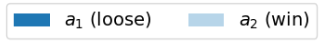
\includegraphics[width=0.2\textwidth]{abig/bd_optim/legend_small_ABIM.png}\\
    \begin{tabular}{cccccccc}
        \includegraphics[width=0.121\textwidth]{abig/bd_optim/initial_policy.png} &\hspace{-0.4cm}  \includegraphics[width=0.11\textwidth]{abig/bd_optim/policy_0.png} &\hspace{-0.4cm}\includegraphics[width=0.11\textwidth]{abig/bd_optim/policy_2.png} &\hspace{-0.4cm}\includegraphics[width=0.11\textwidth]{abig/bd_optim/policy_3.png} &\hspace{-0.4cm}\includegraphics[width=0.11\textwidth]{abig/bd_optim/policy_4.png} &\hspace{-0.4cm}\includegraphics[width=0.11\textwidth]{abig/bd_optim/policy_5.png}
        &\hspace{-0.4cm}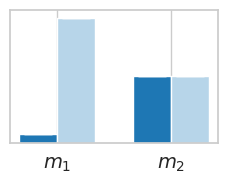
\includegraphics[width=0.11\textwidth]{abig/bd_optim/policy_6.png}
        &\hspace{-0.4cm}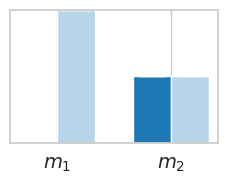
\includegraphics[width=0.11\textwidth]{abig/bd_optim/policy_7.png}\\
        \small $i=0$ & \small \hspace{-0.4cm}$i=1$ & \small \hspace{-0.4cm} $i=2$ & \small \hspace{-0.4cm} $i=3$ &\small \hspace{-0.4cm} $i=4$ &\small \hspace{-0.4cm} $i=5$ &\small \hspace{-0.4cm} $i=6$ &\small \hspace{-0.4cm} $i=7$
    \end{tabular}
    \caption{\abig-driven evolution of message-conditioned action probabilities (builder's policy) for a simple problem where the builder must learn to produce action $a_2$. Even under unfavorable initial condition the architect-builder pair eventually manages to associate a message (here $m_1$) with the winning action ($a_2$). Initial conditions are unfavorable since $a_1$ is more likely than $a_2$ for both messages. ($i=0$) Given the initial conditions, the architect only sends message $m_1$ since it is the most likely to result in action $a_2$. ($i=1$) the builder guiding data only consisted of $m_1$ message therefore it cannot learn a preference over actions for $m_2$ and both actions are equally likely under $m_2$. The architect now only sends message $m_2$ since it is more likely than $m_1$ at triggering $a_2$. ($i=2$) Unfortunately, the sampling of $m_1$ resulted in the builder doing more $a_1$ than $a_2$ during the guiding frame and the builder thus associates $m_2$ with $a_1$. The architect tries its luck again but now with $m_1$. ($i=3$) Eventually, the sampling results in more $a_2$ actions being sampled in the guiding data and the builder now associates $m_1$ to $a_2$. ($i=4$) and ($i=5$) The architect can now keep on sending $m_1$ messages to reinforce this association.}
    \label{fig:bd_optim}
\end{figure}
%
\begin{figure}[h!]
    \centering
    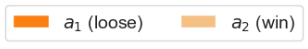
\includegraphics[width=0.2\textwidth]{abig/bd_random/legend.png}
    \begin{tabular}{ccccccc}
        \includegraphics[width=0.143\textwidth]{abig/bd_random/initial_policy.png} &\hspace{-0.4cm}  \includegraphics[width=0.13\textwidth]{abig/bd_random/policy_0.png} &\hspace{-0.4cm} 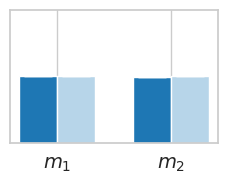
\includegraphics[width=0.13\textwidth]{abig/bd_random/policy_1.png} &\hspace{-0.4cm}\includegraphics[width=0.13\textwidth]{abig/bd_random/policy_2.png} &\hspace{-0.4cm}\includegraphics[width=0.13\textwidth]{abig/bd_random/policy_3.png} &\hspace{-0.4cm}\includegraphics[width=0.13\textwidth]{abig/bd_random/policy_4.png} &\hspace{-0.4cm}\includegraphics[width=0.13\textwidth]{abig/bd_random/policy_5.png}
    \end{tabular}
    \caption{\abig-no-intent driven evolution of message-conditioned action probabilities for a simple problem where builder must learn to produce action $a_2$. Initial conditions are unfavorable since $a_1$ is more likely than $a_2$ for both messages. Without an architect's guiding messages during training, a self-imitating builder reinforces the action preferences of the initial conditions and fails (even when evaluated alongside a knowledgeable architect as both messages can only yield $a_1$).}
    \label{sup:fig_bd_radom}
\end{figure}

To further assess how the architect's message choices impact the performance of a self-imitating builder, we compare the distribution of the builder's preferred actions obtained after using \abig and \abig-no-intent. We consider three different initial conditions (favorable, unfavorable, intermediate) that are each ran to convergence (meaning that the policy does not change anymore across iterations) for 100 different seeds.  Figure~\ref{sup:fig_res_toy} displays the resulting distributions of preferred -- i.e. most likely -- action for each message. When applying \abig on the toy problem, the pair always reaches a success rate of 100/100 no matter the initial condition. We also observe that -- at convergence -- the builder never prefers action $a_1$, yet when an action is preferred for a given message, the other message yields no preference over action ($p(a_1|m)=p(a_2|m)$). This is due to the forget mechanism discussed in Section~\ref{sec:intuition}. The results when applying \abig-no-intent on the toy problem are much more dependent on the initial condition. In the unfavorable scenario, \abig-no-intent fails heavily with only 3 seeds succeeding over the 100 experiments. This is due to the fact that, in absence of message guidance from the architect, the builder has high chances to continually reinforce the association between the two messages and $a_1$, therefore losing. However, in rare cases, the builder can inverse the initial message-conditioned probabilities by 'luckily' sampling more often $a_2$ when receiving $m_1$ and win. This only happened 3 times over the 100 seeds. Finally, when initial conditions are more favorable, the self-imitation  steps reinforce the association between the messages and $a_2$ which makes the builder prefer $a_2$ for at least one message and enables high success rates (100/100 for favorable and 98/100 for intermediate).
%
\begin{figure}[h!]
    \scriptsize{
     \begin{tabular}{ccc}
        \small Unfavorable & \small Favorable & \small Intermediate\\
        \hline
        \\
        \multicolumn{3}{c}{\small (a) \textbf{Initial probabilities}}\\
        \\
        $P(a_1|m_1) = 0.8$, $P(a_2|m_1)=0.2$ & $P(a_1|m_1) = 0.2$, $P(a_2|m_1)=0.8$ & $P(a_1|m_1) = 0.9$, $P(a_2|m_1)=0.1$ \\
        $P(a_1|m_2) = 0.9$, $P(a_2|m_2)=0.1$ & $P(a_1|m_2) = 0.1$, $P(a_2|m_2)=0.9$ & $P(a_1|m_2) = 0.1$, $P(a_2|m_2)=0.9$ \\
        \\
        \hline
        \\
        \multicolumn{3}{c}{\small (b) \textbf{\abig: } Distributions of final preferred action for each message calculated over 100 seeds} \\
        \\
        &  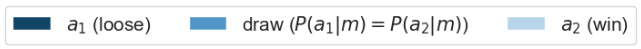
\includegraphics[width=0.3\textwidth]{abig/toy_prob/legend_ABIM.png} & \\
        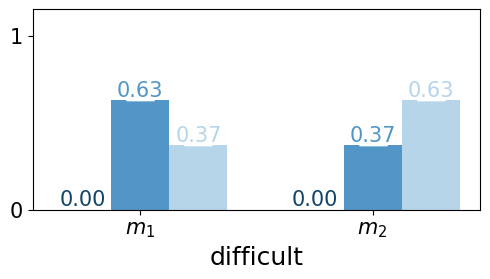
\includegraphics[width=0.3\textwidth]{abig/toy_prob/toy_prob_freq_ABIM_difficult.png} & 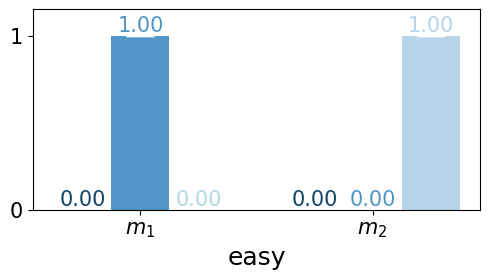
\includegraphics[width=0.3\textwidth]{abig/toy_prob/toy_prob_freq_ABIM_easy.png} &
        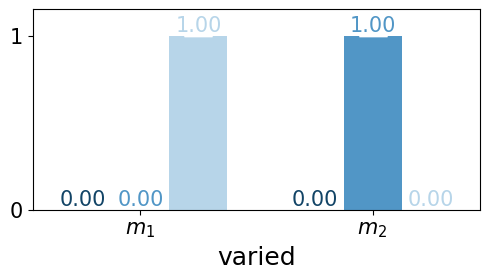
\includegraphics[width=0.3\textwidth]{abig/toy_prob/toy_prob_freq_ABIM_varied.png}\\
        Success Rate = 100/100 & Success Rate = 100/100 &  Success Rate = 100/100\\
        \\
        \hline
        \\
        \multicolumn{3}{c}{\small (c) \textbf{\abig-no-intent: } Distributions of final preferred action for each message calculated over 100 seeds }\\
        \\
        &  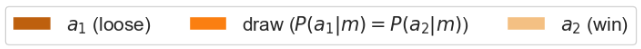
\includegraphics[width=0.3\textwidth]{figures/abig/toy_prob/legend_ABIM-no-intent} & \\
        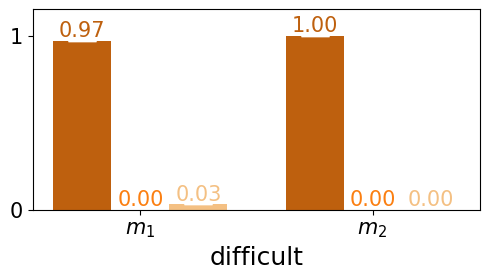
\includegraphics[width=0.3\textwidth]{abig/toy_prob/toy_prob_freq_ABIM-no-intent_difficult.png} & 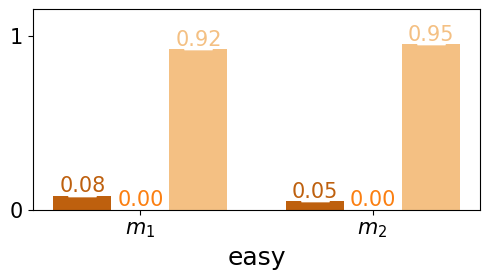
\includegraphics[width=0.3\textwidth]{abig/toy_prob/toy_prob_freq_ABIM-no-intent_easy.png} &
        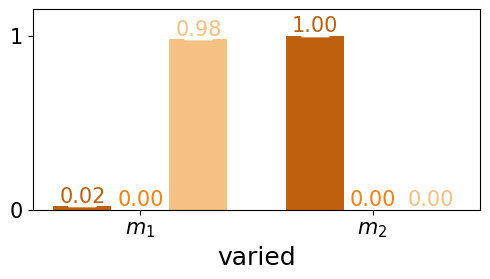
\includegraphics[width=0.3\textwidth]{abig/toy_prob/toy_prob_freq_ABIM-no-intent_varied.png}\\\
        Success Rate = 3/100 & Success Rate = 100/100 & Success Rate = 98/100\\
    
    \end{tabular}
    }
    \caption{\textbf{Toy experiment analysis} (a) Initial conditions: initial probability for each action $a$ given a message $m$; distributions of final builder's preferred actions for each message after applying (b) \abig and (c) \abig-no-intent on the toy problem; distributions are calculated over 100 seeds. For each method and each initial condition, we report the success rate obtained by a knowledgeable architect guiding the builder. At evaluation, the architect has access to the builder's model and does not ignore the goal. \abig always succeeds while \abig-no-intent's success depends on the initial conditions.}
    \label{sup:fig_res_toy}
\end{figure}

\newpage

\subsection{Related Work}
\label{ap:sec_related_work}
In this section we develop the differences between \abp and Hierarchical/Feudal Reinforcement Learning more in detail.

\cite{kulkarni2016hierarchical} proposes to decompose a RL agent into a two-stage hierarchy with a meta-controller (or manager) setting the goals of a controller (or worker). The meta-controller is trained to select sequences of goals that maximize the environment reward while the controller is trained to maximize goal-conditioned intrinsic rewards. The definition of the goal-space as well as the corresponding hard-coded goal-conditioned reward functions are task-related design choices. In \cite{vezhnevets2017feudal}, the authors propose a more general approach by defining goals as embeddings that directly modulate the worker's policy. Additionally, the authors define intrinsic rewards as the cosine distance between goals and embedded-state deltas (difference between the embedded-state at the moment the goal was given and the current embedded-state). Thus, goals can be interpreted as directions in embedding space.
\cite{nachum2018data} build on a this idea but let go of the embedding transformation by considering goals as directions to reach and rewards as distances between state deltas and goals. 
These works tackle the single-agent learning problem and therefore allow the manager to directly influence the learning signal of the workers. However, in the multi-agent setting where agents are physically distinct, it is not possible for an agent to explicitly tweak another agent's learning algorithm. Instead, agents must communicate by influencing each other's observations instead of intrinsic rewards. Since it is designed to investigate the emergence of communication between agents, \abp lies in this latter multi-agent setting where agents can interact with one-another only through observations. This makes applying Feudal or Hierarchical methods to the \abp unfeasible as they are restricted to worker agents that directly receive rewards. In contrast, in \abp, the reward-less builder observes communication messages that, initially, have arbitrary meaning.  



\newpage \section{Supplementary Results}
%
\label{ap:sup_res}
\subsection{Learning Analysis}
\label{ap:results_bw}
The main document shows performances (success rates) of builder-architect pairs at convergence. In this supplementary section we propose to thoroughly study the evolution of the builder's policy in order to provide a deeper analysis of \abig.

\textbf{Metric definition. } We define three metrics that characterize the builder behavior. We compute these metrics on a constant \emph{Measurement Set} $\mathcal{M}$ made of 6000 randomly sampled states, for each of these states we sample all the possible messages $m\sim$ Uniform($\gV$) where $\gV$ is the set of possible messages. Therefore, $|\gM| = 6000\times|\gV|$. The set of possible actions is $\gA$ and we denote by $\delta$ the indicator function.\\

We also define the following distributions:
 \begin{align*}
     &\ps(s) \triangleq \frac{1}{|\gM|}\sum_{s'\in\gM}\delta(s'==s)\\
     &\pM(m) \triangleq P(m|s) =  \frac{1}{|\gV|}\\
     &\psm(s,m) \triangleq \ps(s)P(m|s) = \ps(s)\pM(m)\\
     &\psma(s,m,a) \triangleq \psm(s,m)P(a|s,m) = \psm(s,m)\pib(a|s,m)\\
    & \pa(a) \triangleq \sum_{(s,m)\in \gM} \psma(s,m,a)\\
     &\pma(m,a)\triangleq \sum_{s\in\gM}\psma(s,m,a)\\
     &\psa(s,a)  \triangleq \sum_{m\in\gM}\psma(s,m,a)
 \end{align*}
From this we can define the monitoring metrics:
\begin{itemize}
    % \item \textit{Policy similarity: } This metric is defined as the accuracy between the preferred action distribution of two of two policies. 
    % $$\text{sim}(\pi_1,\pi_{2})=\frac{1}{\mathcal{|M|}}\sum_{(s,m)\in \mathcal{M}} (\argmax{\pi_{1}(s,m)}==\argmax{\pi_2(s,m)})$$
    \item \textit{Mean Entropy: }
    $$\bar{H}(\pi)=\frac{1}{|\gM|}\sum_{(s,m)\in \mathcal{M}} \left[ - \sum_{a\in \gA}\pi(a|s,m)\text{log}\pi(a|s,m)\right]$$ 
    \item \textit{Mutual Information between messages and actions}
    $$I_m = \sum_{m\in \gV}\sum_{a\in \gA}\pma(m,a)\log\frac{\pma(m,a)}{\pa(a)\pM(m)}$$
    \item \textit{Mutual Information between states and actions}
    $$I_s = \sum_{s\in \gM}\sum_{a\in \gA}\psa(s,a)\log\frac{\psa(s,a)}{\pa(a)\ps(s)} $$
\end{itemize}

\textbf{Analysis. } Figure~\ref{sup:fig_learning_metrics} displays the evolution of these metrics after each iteration as well as the evolution of the success rate (a). As indicated by Eq.~(\ref{eq:bc_entropy}), doing self-imitation learning results in a decay of the mean entropy (b). This decay is similar for \abig and \abig-no-intent. The most interesting result is provided by the evolution of the mutual information (c). For \abig-no-intent, we see that $I_s$ and $I_m$ slowly increase with $I_s>I_m$ over all iterations. This indicates that the builder policy $\pi_B(a|s,m)$ relies more on states than on messages to compute the actions. In this scenario the builder, therefore, tends to ignore messages. On the other hand, $I_s$ and $I_m$ evolve differently for \abig. Both metrics first increase with $I_s>I_m$ until they cross around iteration $25$. Then $I_s$ starts decreasing and $I_m$  grows. This shows that \abig results in a builder policy that strongly selects actions based on the messages it receives which is a desirable feature of emergent communication.  

\begin{figure}[h!]
    \centering
    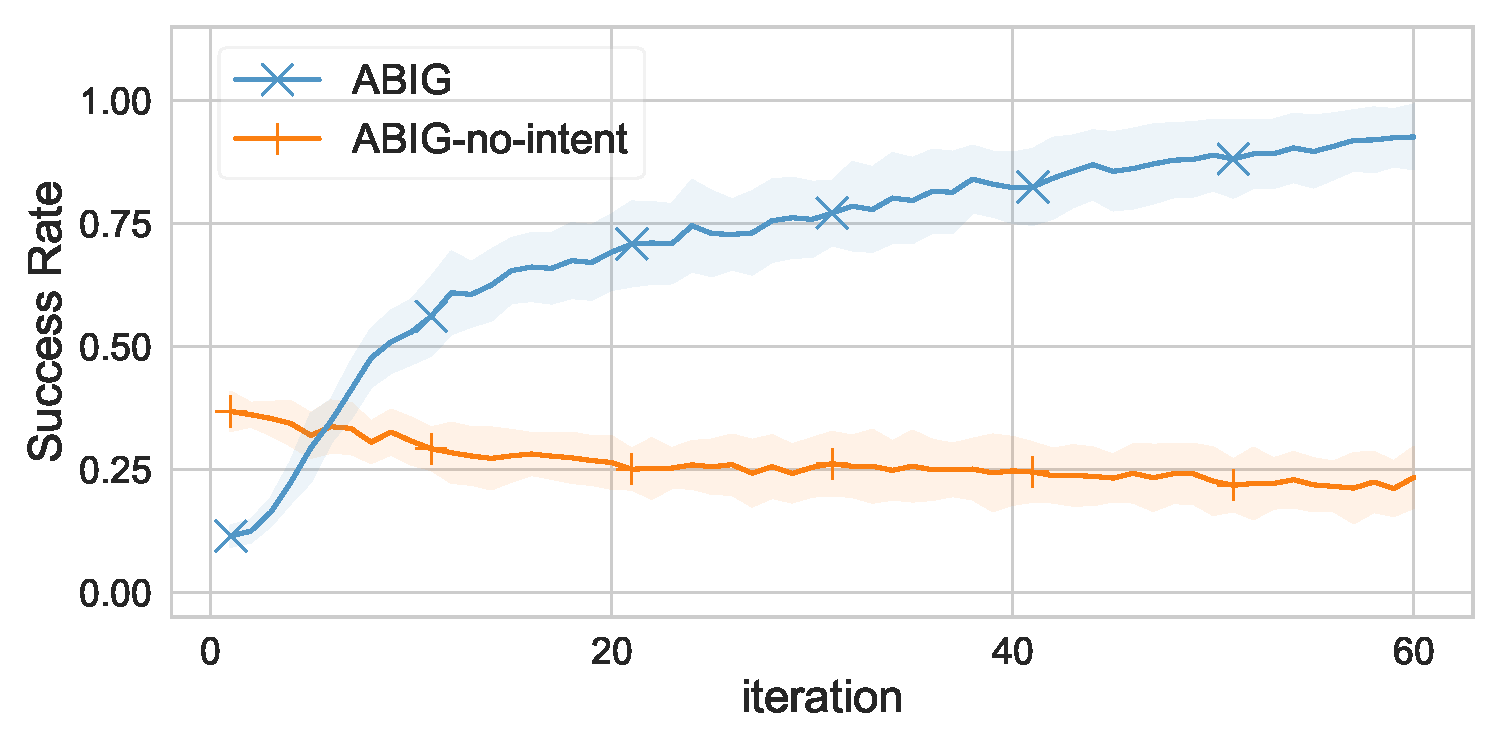
\includegraphics[width=0.6\textwidth]{abig/learning_success.pdf}\\
    \small(a) Evolution of the success rate\\
    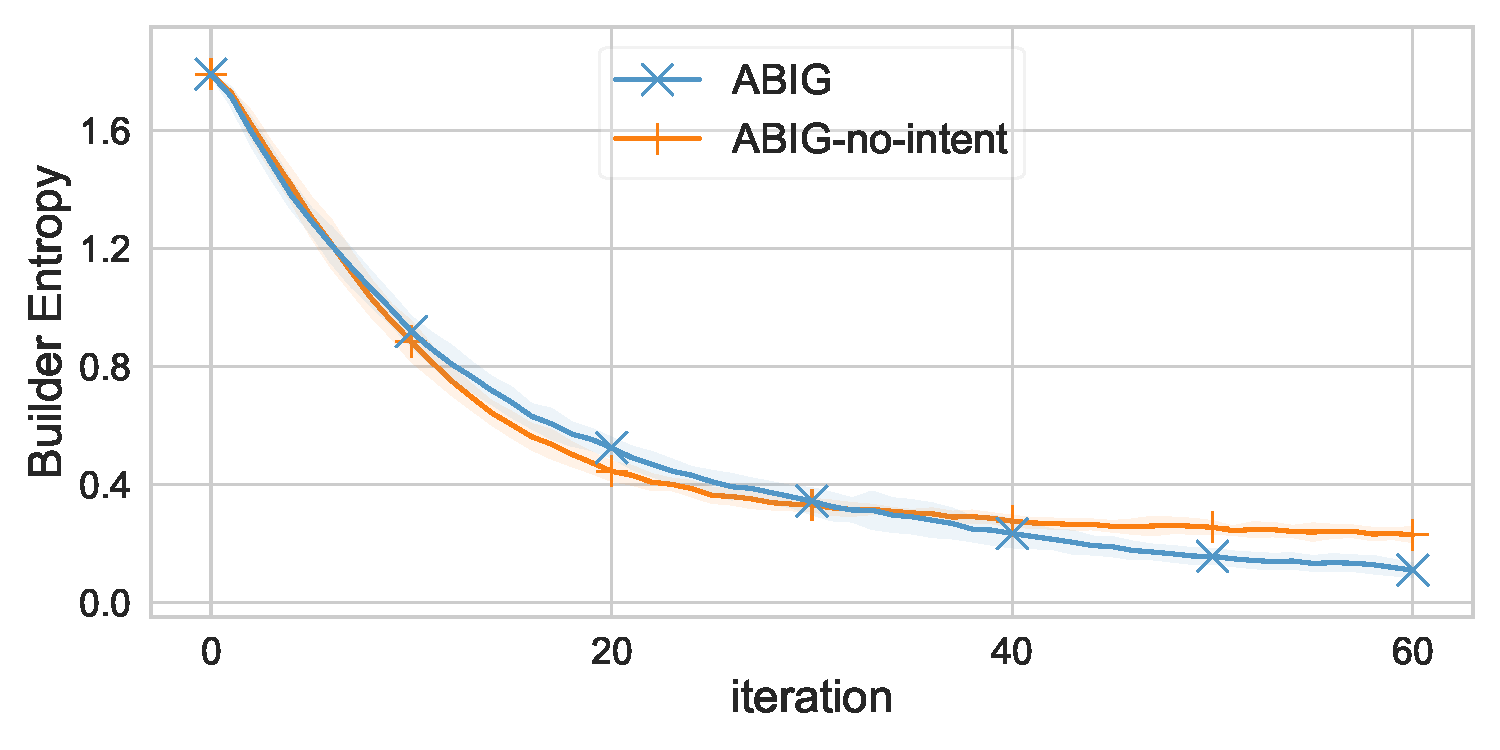
\includegraphics[width=0.6\textwidth]{abig/learning_entropy.pdf}\\
    \small(b) Evolution of the builder policy mean entropy $\bar{H}_{\pi_B}$\\
    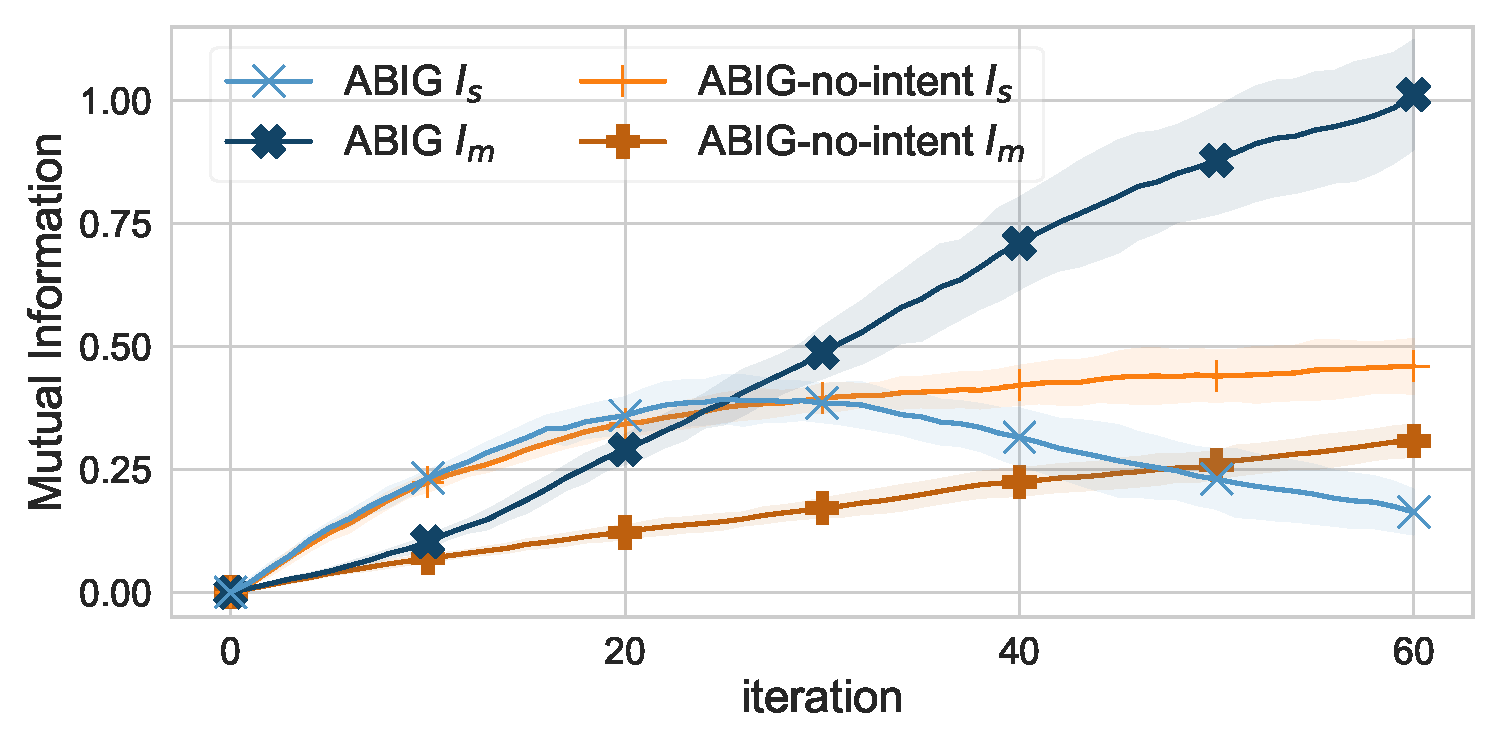
\includegraphics[width=0.6\textwidth]{abig/learning_MI.pdf}\\
    \small(c) Evolution of the mutual information $I_s$ and $I_m$
    \caption{Comparison of the evolution of builder policy properties when applying \abig and \abig-no-intent on the 'place' task in BuildWorld. (a) \abig enables much higher performance that \abig-no-intent. (b) Both methods use self-imitation and thus reduce the entropy of the policy. (c) \abig promotes the mutual information between messages and action which indicates successful communication protocols.}
    \label{sup:fig_learning_metrics}
\end{figure}

\subsection{Additional Baseline Comparison}
\label{ap:baselines}
We define two extra baselines: 
\begin{itemize}[noitemsep]
    \item Stochastic: where the builder policy is a fixed softmax policy parameterized by a randomly initialized network;
    \item Deterministic: where the builder policy is a fixed argmax policy parameterized by a randomly initialized network.
\end{itemize}
In the performances reported in Figure~\ref{fig:baseline_performance}, the architect has direct access to the exact policy of the builder ($\tildepib=\pib$) and uses it to plan and guide the builder during evaluation.  We observe that the stochastic condition exhibits similar performances as the random builder. This indicates that, even if the architect tries to guide the builder, the stochastic policy is not controllable and performances are not improved. Finally, we would expect a deterministic policy to be more easily controllable by the architect. Yet, as pointed out in Figure~\ref{fig:baseline_performance}, the initial deterministic policies lack flexibility and fail. This shows that the builder must iteratively evolve its policy in order to make it controllable.

\begin{figure}[h!]
    \centering
    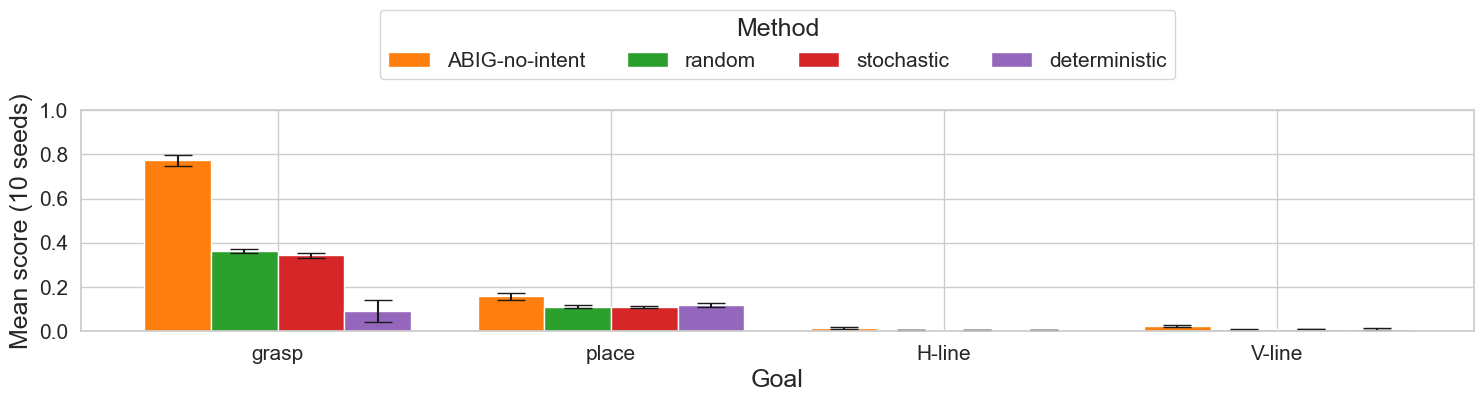
\includegraphics[width=1.\textwidth]{abig/performance_baselines_dict_size18.png}
    \caption{Baseline performance depending on the goal: stochastic policy behaves on par with random builder. Self-imitation with \abig-no-intent remains the most controllable baseline.}
    \label{fig:baseline_performance}
\end{figure}
\subsection{Impact of the Vocabulary Size}
\label{sup:sec_res_dict_size}
\begin{figure}[h!]
    \centering
    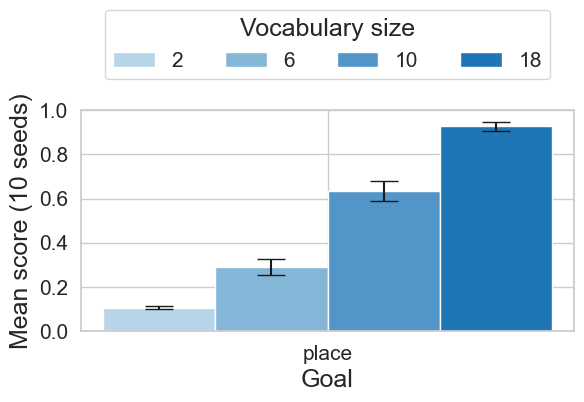
\includegraphics[width=.4\textwidth]{abig/performance_dict_size.png}
    \caption{Influence of the Vocabulary size for \abig on the 'place' task. Performance increases with the vocabulary size.}
    \label{fig:dict_size_performance}
\end{figure}


\end{document}
